\title{Epileptic Seizure Detection from EEG Signals with Denoising Autoencoders}
\author{Tuan Nguyen}
\date{\today}

\documentclass[12pt]{article}

\usepackage{url}
\usepackage{graphicx}
\usepackage{subcaption}
\usepackage{booktabs}
\usepackage{hyperref,xcolor}
\usepackage{listings}

\newcommand{\myvec}[1]{\mathbf{#1}}

\begin{document}
\maketitle

\section{Definition}

\subsection{Project Overview}
\noindent
The domain of interest of this project belongs to physiological data such as electroencephalography (EEG), magnetoencephalography (MEG), electrocardiography (ECG) and the recorded signals from wearable devices. This project focuses on the EEG signals, which capture activities of brain neurons during a period of time. Different kinds of EEG data has been recorded from humans, for instance from those at rest, sleep~\cite{langkvist2012sleep}, during some periods of specific cognitive activities, or from patients with diseases such as Alzheimer's, Parkinson's, depression and epileptic seisures (\cite{andrzejak2001indications} and references thereof).

This project studies the classification problem on an EEG data set recorded from healthy volunteers and patients having epileptic seizures~\cite{andrzejak2001indications}; solutions for this problem could be used to assist with detecting patients with the disease from their brain activity signals. Previous work on this data set focused mainly on extracting hand-crafted features to be used for classification. As examples, Nigam and Graupe \cite{nigam2004neural} extracted the spike amplitudes and frequency of the signals, feeding them into a neural network for classification; Guler et al.~\cite{guler2005recurrent} applied wavelet transformation to the signals to extract features, and classification was performed using a neuro-fuzzy system; Kannathal et al.~\cite{kannathal2005entropies} extracted entropy-based features for classification. Although these approaches resulted in solutions with high accuracy performance, it is still an interesting question as to whether the process of feature learning and classification could be done automatically.

Deep multi-layer neural networks with many levels of non-linearities are capable of compactly represent complex non-linear function, and therefore are powerful machine learning models for dimensionality reduction and feature learning. A great challenge in training those deep ``autoencoders'' networks, however, is that a network with randomly initialized parameters tends to get stuck at poor solutions. Hinton et al.~\cite{hinton2006reducing} showed that Deep Belief Networks, a type of deep networks, initialized using weights from a stack of pretrained Restricted Boltzmann machines (RBMs) could be trained successfully to reduce the dimensionality of data. The strategy of training the RBMs was novel in that it was an \emph{unsupervised} learning to reconstruct corresponding inputs; and the same strategy has also been shown to be applicable for regular deep multi-layer neural networks in which auto-encoders were pretrained and used as building blocks (instead of RBMs)~\cite{bengio2007greedy}. In terms of applying these ideas to EEG signals, on a different data set Wulsin et al.~\cite{wulsin2011modeling} learned features of second-long EEG segments using Deep Belief Networks~\cite{hinton2006reducing} and classified them into ``clinically significant'' EEG classes. To the best of my knowledge, there was no previous work reporting the results of using autoencoders for the data set that this project is interested in. The purpose of this work, therefore, is to explore the use of traditional and denoising autoencoders (\cite{bengio2007greedy}, \cite{vincent2010stacked}) in learning the features representing the EEG signals and then use them to classify unseen brain activity signals into different classes of patients. For classification purpose, the pretrained autoencoders are in two different ways: (1) to initialize a multi-layer fully-connected networks with a softmax output layer that is further fined-tuned, and (2) to extract high level features of the original data which are then used by popular classifiers such as Support Vector Machines and boosting. To the end, I present extensive experiments that show the great benefits of using denoising autoencoders in detecting epileptic seizure from EEG signals.

\subsection{Problem Statement}
\noindent
This project aims to classify 1-second long EEG segments into one of the three classes: (1) healthy volunteers, (2) patients with epileptic seizures disease during seizure-free periods, and (3) patients with the disease during active seizure periods. It can be formally defined as follows.

\begin{itemize}
\item \textbf{Input:} training set $X = \langle \myvec{x}_1, \myvec{x}_2, ..., \myvec{x}_N\rangle$ of $N$ samples, where $\myvec{x}_i$ is a vector of $M$ electrical voltage values recorded in one second by an electrode at a specific point and time; target vector $y = \langle y_1, y_2, ..., y_N \rangle$ where $y_i \in \{1, 2, 3\}$ is the type of volunteers which the sample $\myvec{x}_i$ belong to. In the data set~\cite{andrzejak2001indications}, the targets $1, 2, 3$ respectively correspond to sets of volunteers $A + B$, $C + D$ and $E$.
\item \textbf{Output:} a hypothesis $h$ classifying a sample of $M$ electrical voltage values into one of the volunteer classes $\{1, 2, 3\}$.
\end{itemize}

The formation of the training set $X$ and target $y$ is presented in more details in Section~\ref{sec:data_set}. This project explores the benefits of using autoencoders in learning a representation $f(\myvec{x}_i)$ of signal segments $\myvec{x}_i \in X$ that can be helpful for our classification task at hand; the two types of autoencoders considered in this work are traditional~\cite{bengio2007greedy} and denoising autoencoder~\cite{vincent2010stacked}. The trained parameters of these autoencoders are then used to fine tune multi-layer feed-forward neural network for classification (see Section~\ref{sec:solution}). %Several metrics are used to evaluate the classifiers, discussed in Section~\ref{sec:metric}.

\subsection{Metrics}
\label{sec:metric}
The purpose of a hypothesis returned for the problem stated above is to classify unseen brain activity segments, correctly as frequently as possible, into one of the volunteer classes $\{1, 2, 3\}$. The \textit{accuracy} is the most important measure for this purpose. Given a hypothesis $h$ and a set of examples $T$, let $C_k(h,T)$ be the number of examples in $T$ classified into correct class $k$ ($k \in \{1,2,3\}$) by $h$. The accuracy of $h$ on the set $T$ is formally defined as follows:

\[Acc(h, T) = \frac{\sum_{k\in\{1,2,3\}}C_k(h,T)}{|T|}.\]

The accuracy measure is used on both the training set to update parameters of a model under construction and the validation set to approximate the performance of the model on future unseen data set. Candidate models are ranked based on their accuracy on an independent test set.

%The quality of the returned hypothesis is evaluated on an independent test set using the accuracy measure, which is the percentage of samples classified into their correct classes. The test set is created from randomly chosen $20\%$ of the given data set. Although, as suggested by Wulsin et al.~\cite{wulsin2011modeling}, the classification time is considered important for applications monitoring EEG signals of patients, the testing set is small enough that the prediction time performed by the multi-layer neural network classifiers is much less than 1 second and therefore will not be discussed further in the result section. (I also regret to note that my implementation did not initially put in tensors for recording the $F_1$ score, which should also be a meaningful measure to examine.)

\section{Analysis}

\subsection{Data Exploration and visualization}

\label{sec:data_set}
The data set used in this study is provided with the work by Andrzejak et al.~\cite{andrzejak2001indications}, recording brain electrical activity of five sets of human volunteers:
\begin{itemize}
\item Set A: healthy volunteers in relaxed state with eyes open.
\item Set B: healthy volunteers in relaxed state with eyes closed.
\item Set D: epilepsy patients during seizure-free periods; the electrodes were implanted to record brain activity from within the epileptogenic zone.
\item Set C: epilepsy patients during seizure-free periods; the electrodes were implanted from the opposite hemisphere of the brain (compared to those in Set D).
\item Set E: same patients with sets C and D but activity were recorded from all electrodes during active seizures.
\end{itemize}

For each set of volunteers above, the data set contains 100 single-channel EEG segments of $4096$ signal micro-Voltage values in time domain of 23.6-sec duration. For this project each of these segments is divided into smaller segments of 1-second durations, which are considered stationary for EEG data~\cite{nigam2004neural}. These 1-second durations together define the training set $X$ of $178$ dimensions, and the three sets of volunteers $A + B$, $C + D$ and $E$ define the target vector $y$ in the problem statement above.

Figure~\ref{fig:signals} shows four randomly chosen 23.6-second segments of each class from which we can only observe very slightly differences in patterns of the signals in each class. However, by looking at the shape of each class more closely it is interesting to notice some very distinguished segments that belong to epileptic seizure patients in both seizure-free or seizure-active periods (i.e., class C, D and E), as shown in Figure~\ref{fig:odd_signals}. We can observe that some signals that belong to patients during their seizure-active periods (i.e., class E) are very dense, whereas classes C and D contain some signals that are more sparse but also include several high peaks within one second.

\begin{figure}
\begin{subfigure}{.25\textwidth}
  \centering
  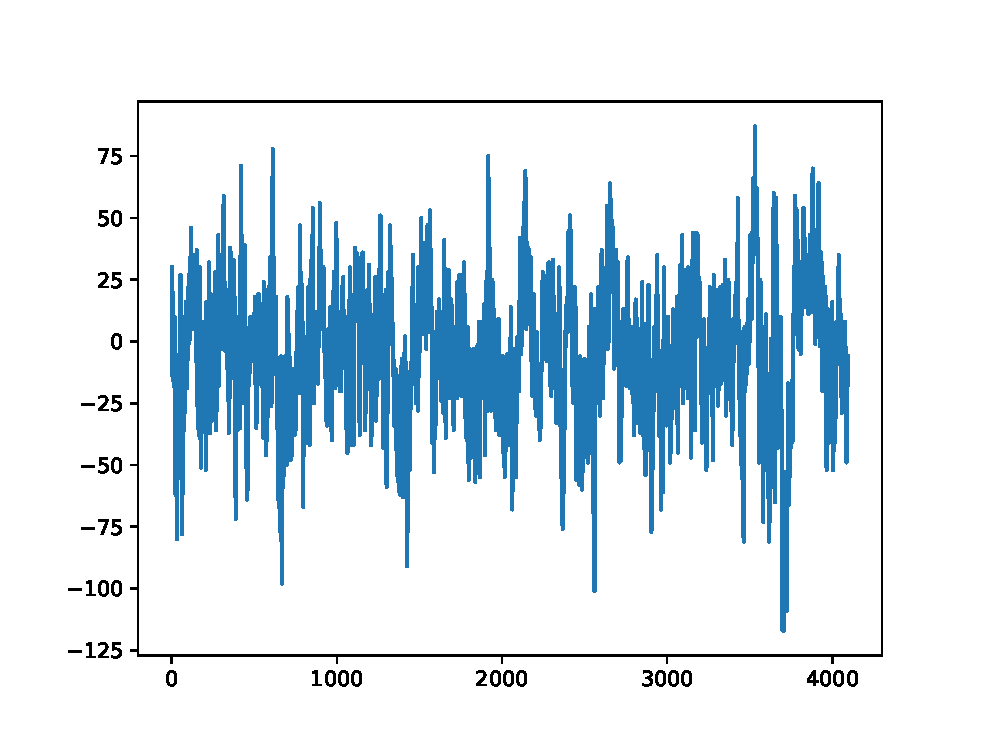
\includegraphics[width=.8\linewidth]{figures/signals/A/Z015.eps}
\end{subfigure}%
\begin{subfigure}{.25\textwidth}
  \centering
  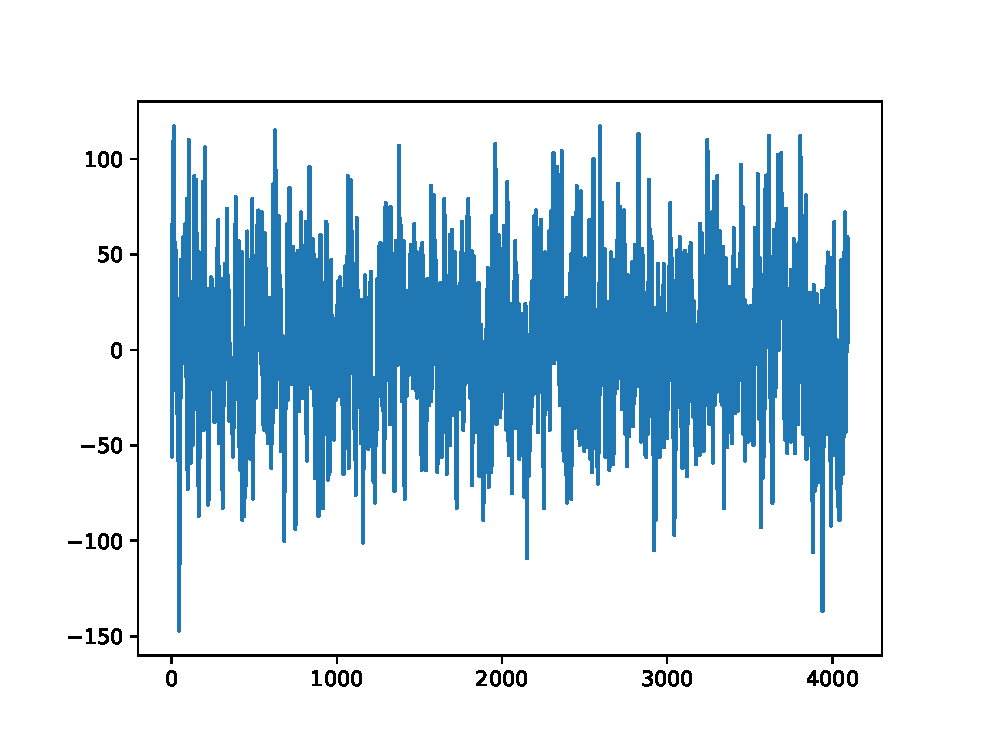
\includegraphics[width=.8\linewidth]{figures/signals/A/Z024.eps}
\end{subfigure}
\begin{subfigure}{.25\textwidth}
  \centering
  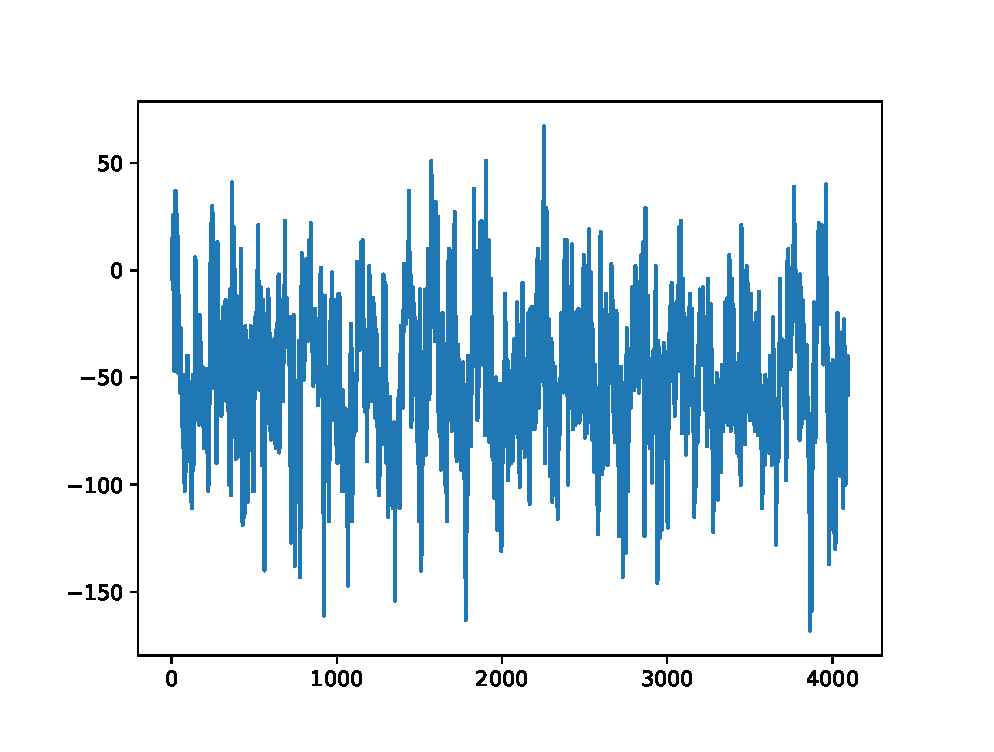
\includegraphics[width=.8\linewidth]{figures/signals/A/Z028.eps}
\end{subfigure}%
\begin{subfigure}{.25\textwidth}
  \centering
  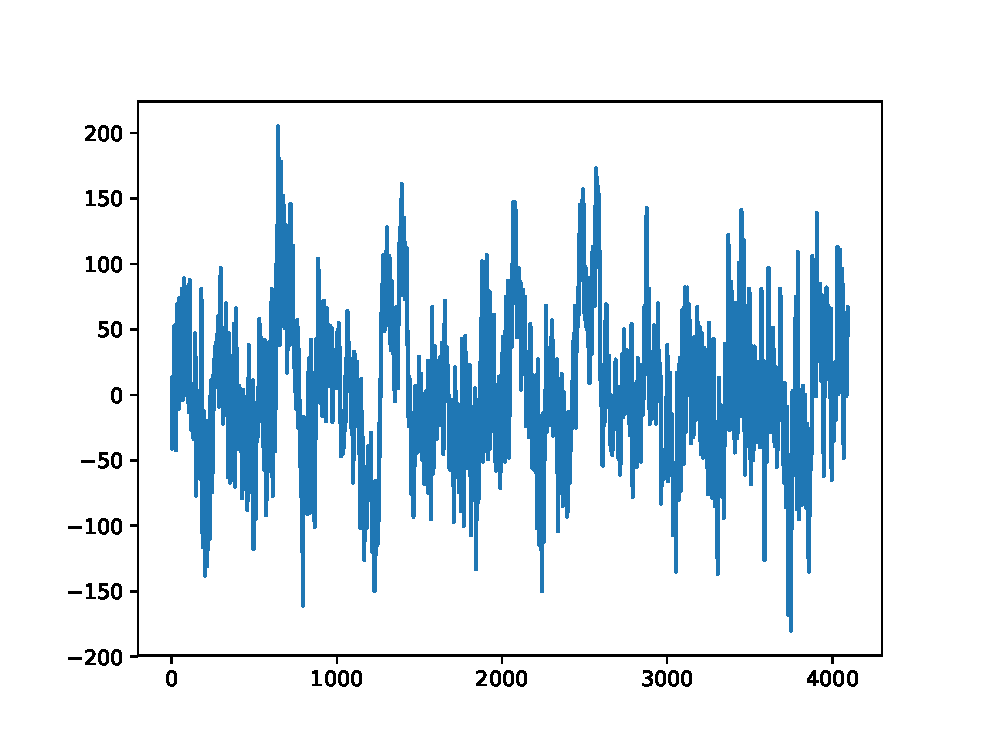
\includegraphics[width=.8\linewidth]{figures/signals/A/Z035.eps}
\end{subfigure}

\begin{subfigure}{.25\textwidth}
  \centering
  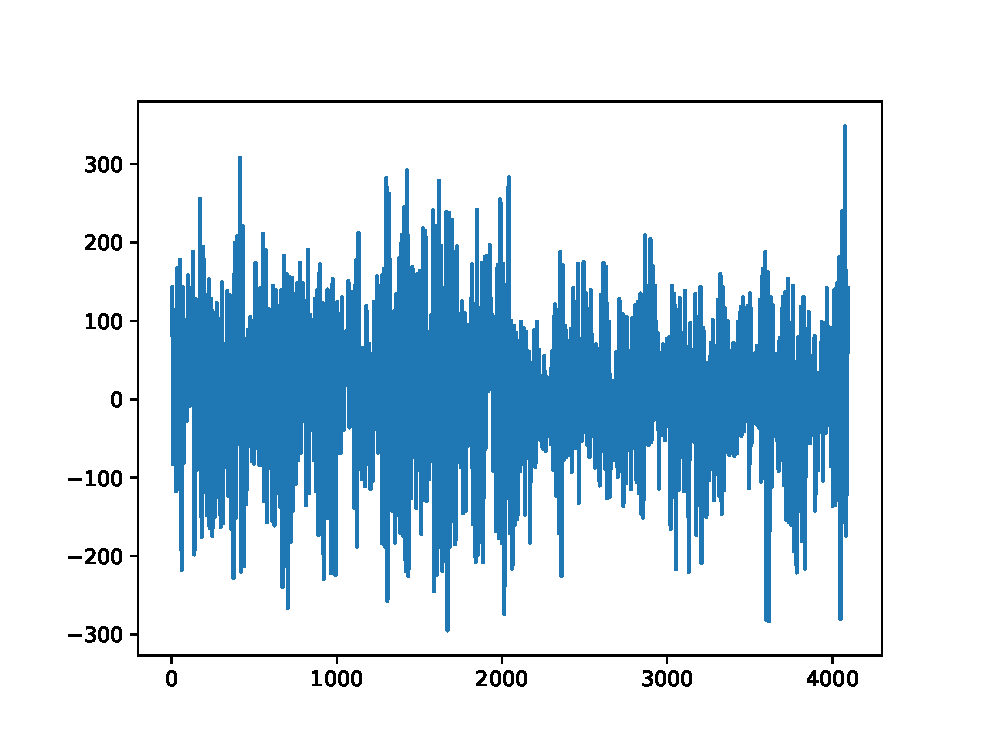
\includegraphics[width=.8\linewidth]{figures/signals/B/O015.eps}
\end{subfigure}%
\begin{subfigure}{.25\textwidth}
  \centering
  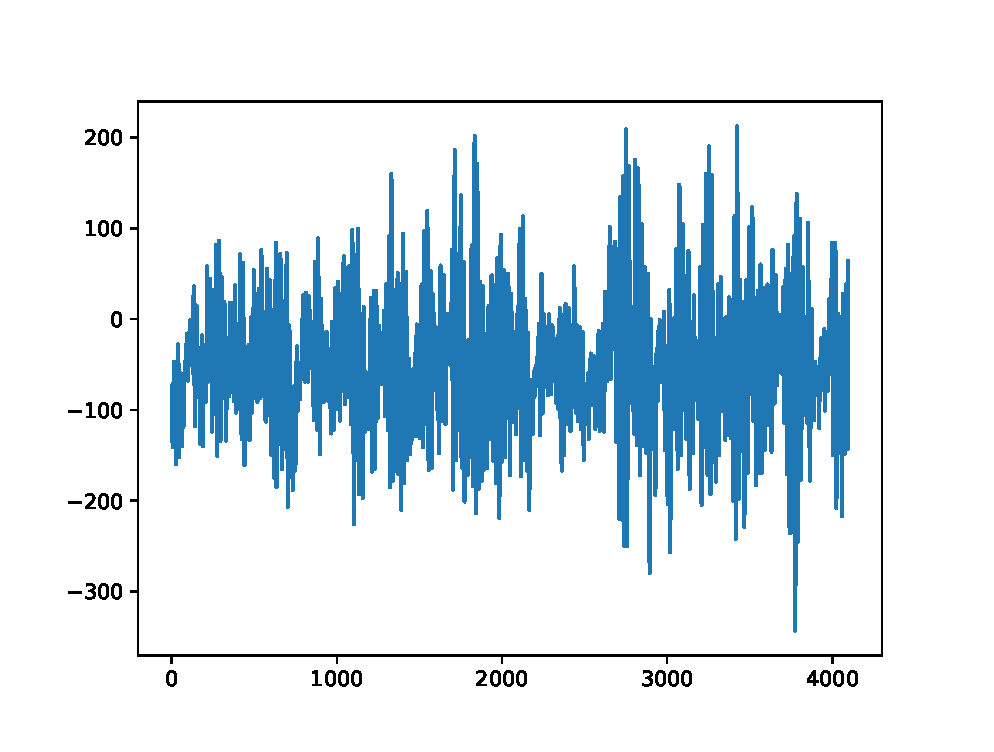
\includegraphics[width=.8\linewidth]{figures/signals/B/O024.eps}
\end{subfigure}
\begin{subfigure}{.25\textwidth}
  \centering
  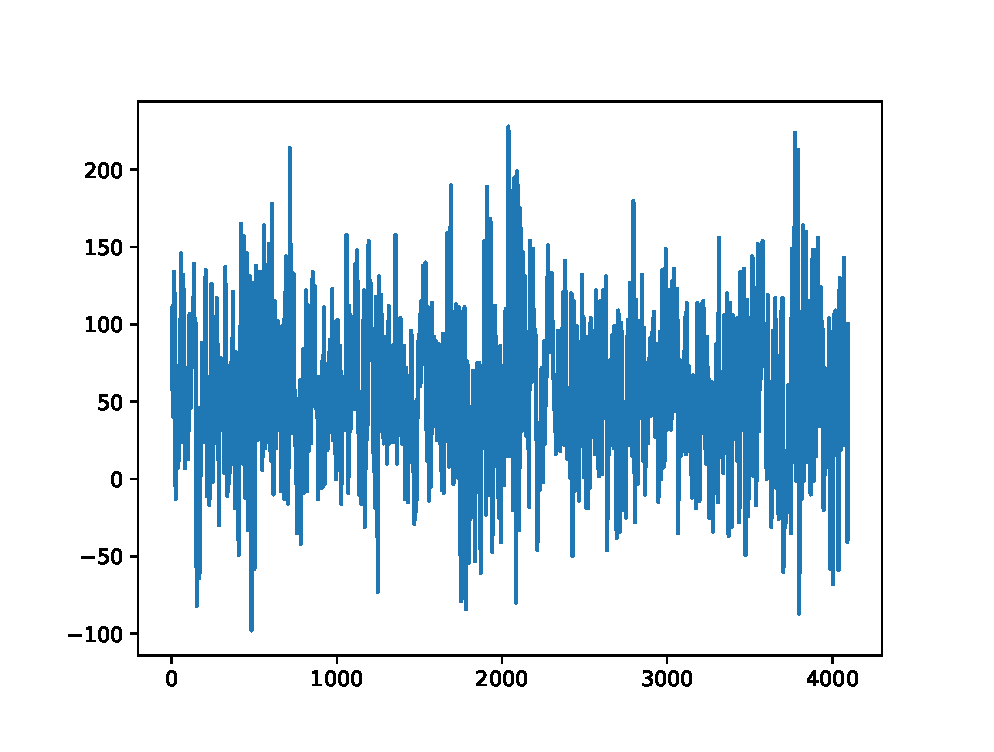
\includegraphics[width=.8\linewidth]{figures/signals/B/O028.eps}
\end{subfigure}%
\begin{subfigure}{.25\textwidth}
  \centering
  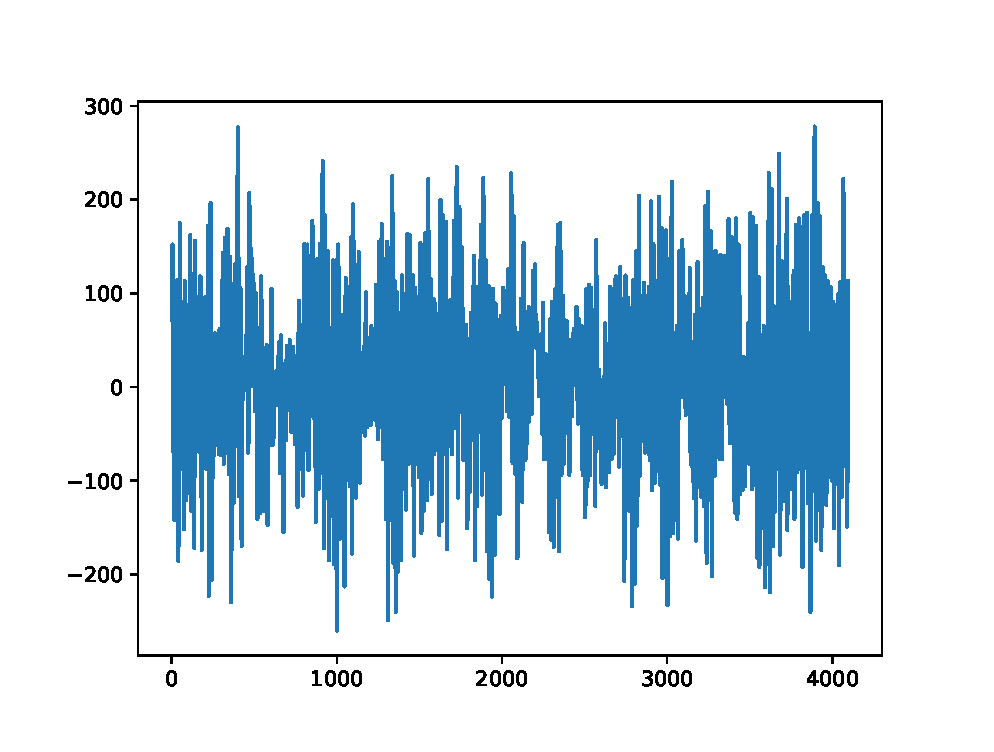
\includegraphics[width=.8\linewidth]{figures/signals/B/O035.eps}
\end{subfigure}

\begin{subfigure}{.25\textwidth}
  \centering
  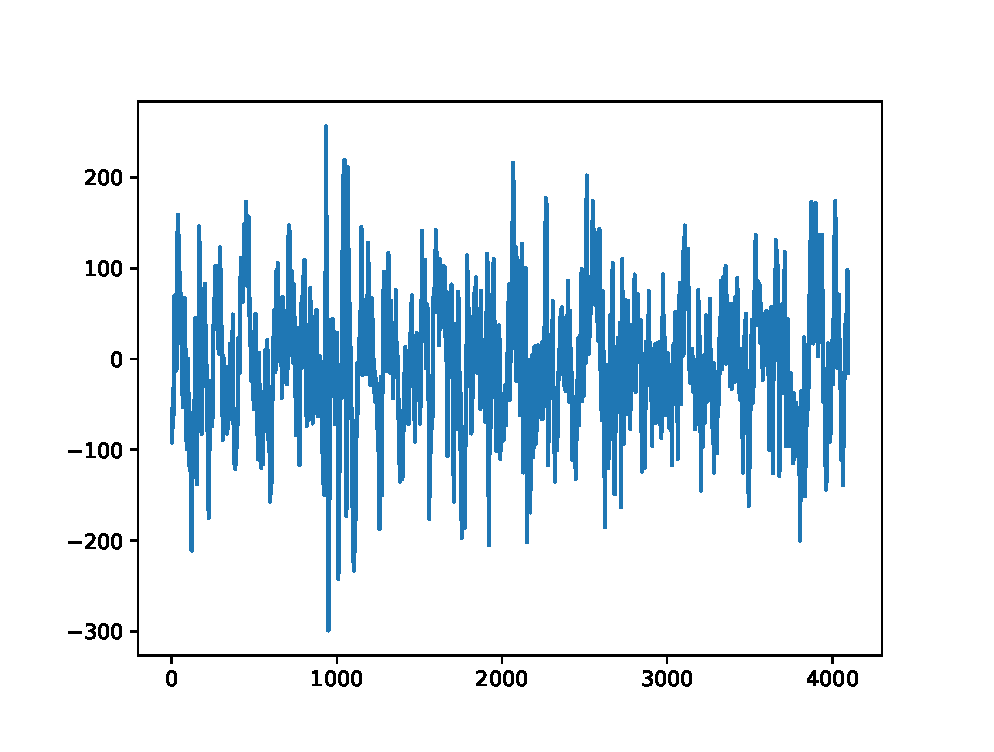
\includegraphics[width=.8\linewidth]{figures/signals/C/N015.eps}
\end{subfigure}%
\begin{subfigure}{.25\textwidth}
  \centering
  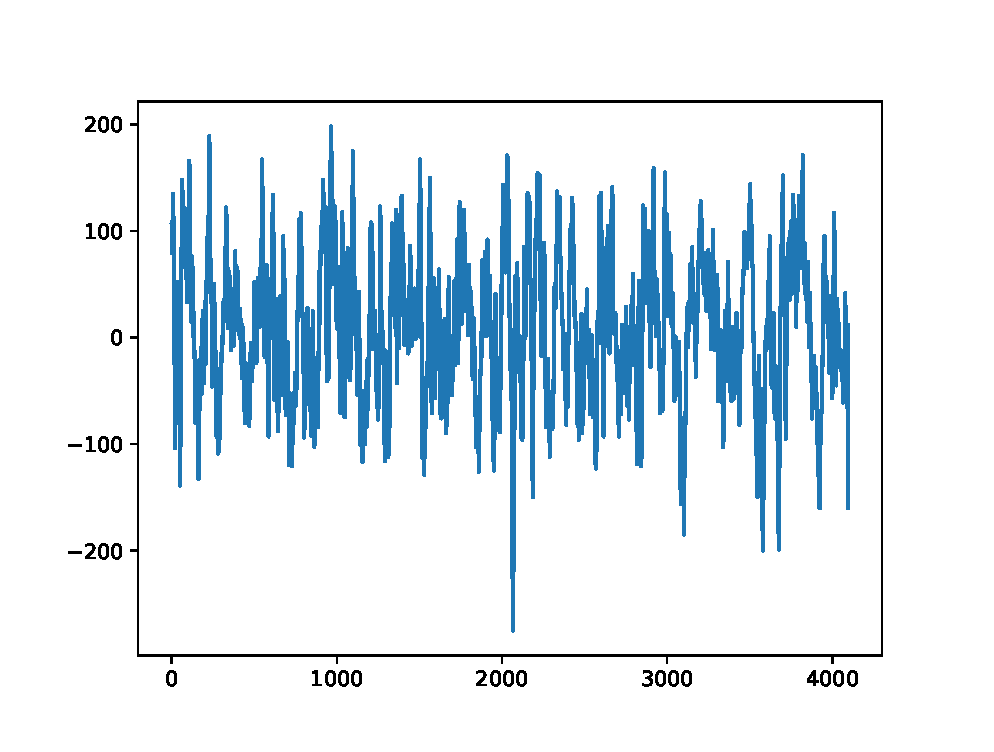
\includegraphics[width=.8\linewidth]{figures/signals/C/N024.eps}
\end{subfigure}
\begin{subfigure}{.25\textwidth}
  \centering
  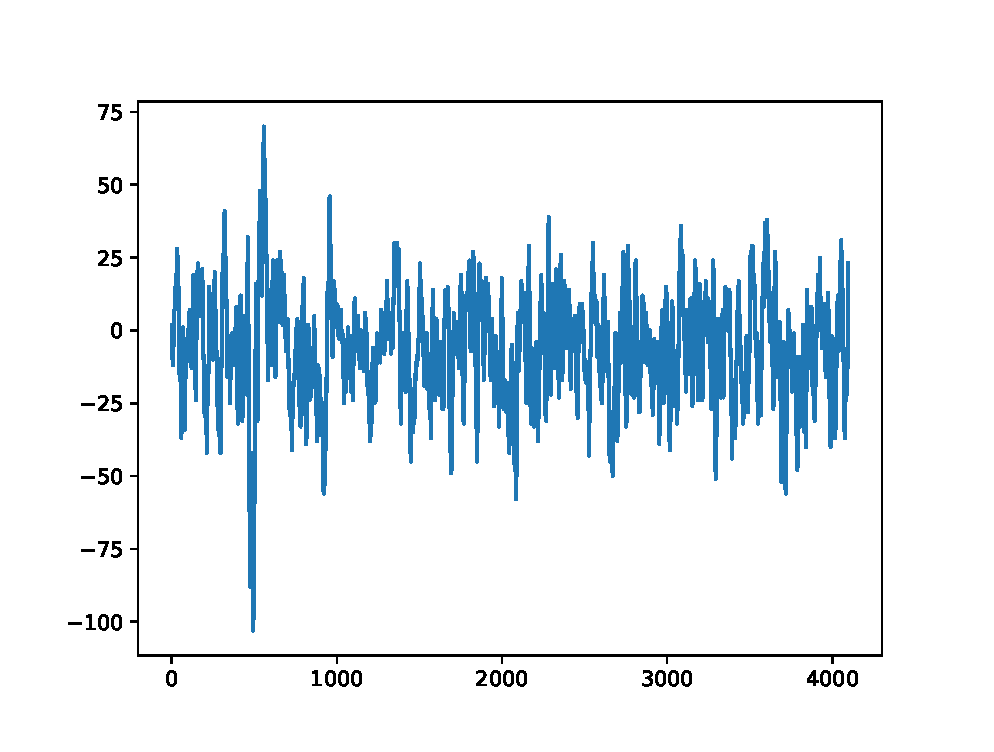
\includegraphics[width=.8\linewidth]{figures/signals/C/N028.eps}
\end{subfigure}%
\begin{subfigure}{.25\textwidth}
  \centering
  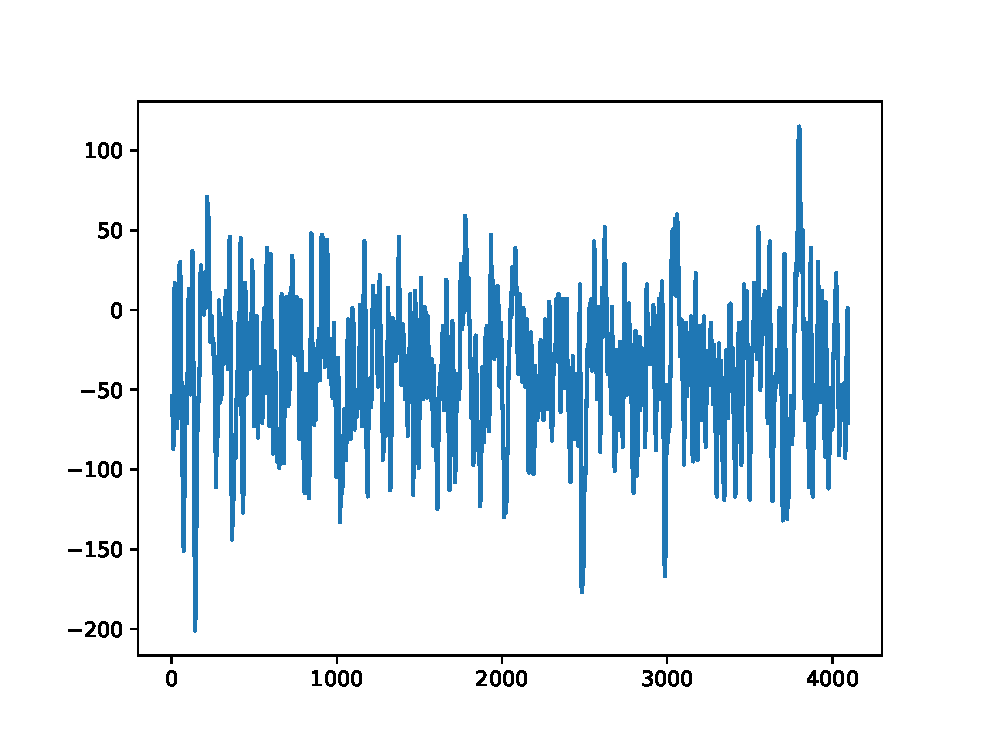
\includegraphics[width=.8\linewidth]{figures/signals/C/N035.eps}
\end{subfigure}

\begin{subfigure}{.25\textwidth}
  \centering
  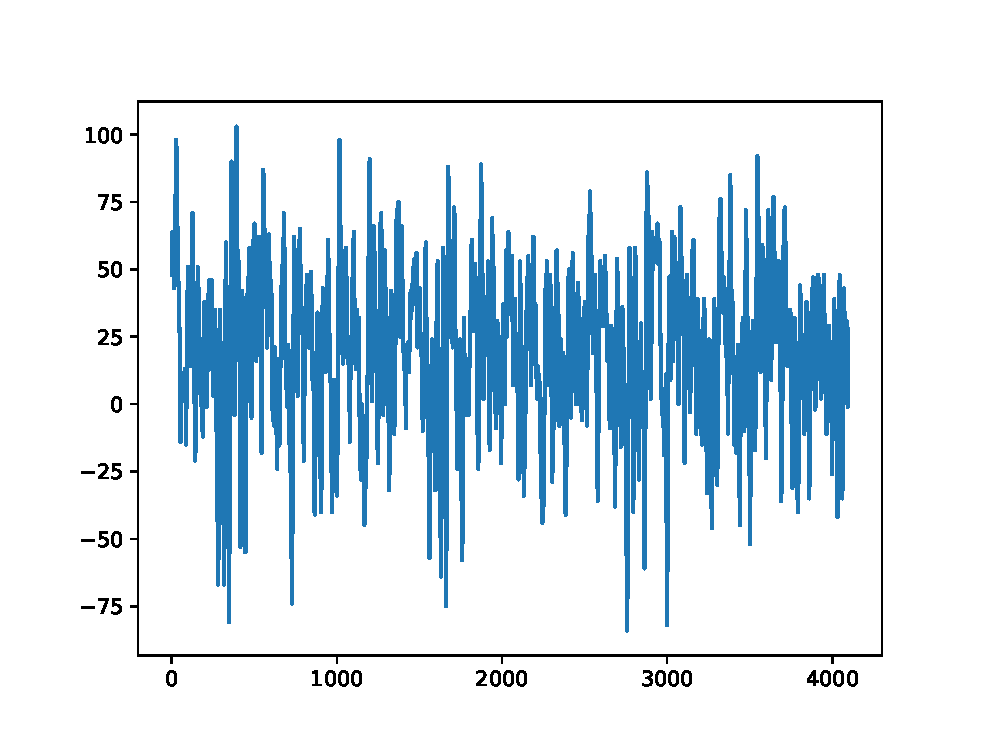
\includegraphics[width=.8\linewidth]{figures/signals/D/F015.eps}
\end{subfigure}%
\begin{subfigure}{.25\textwidth}
  \centering
  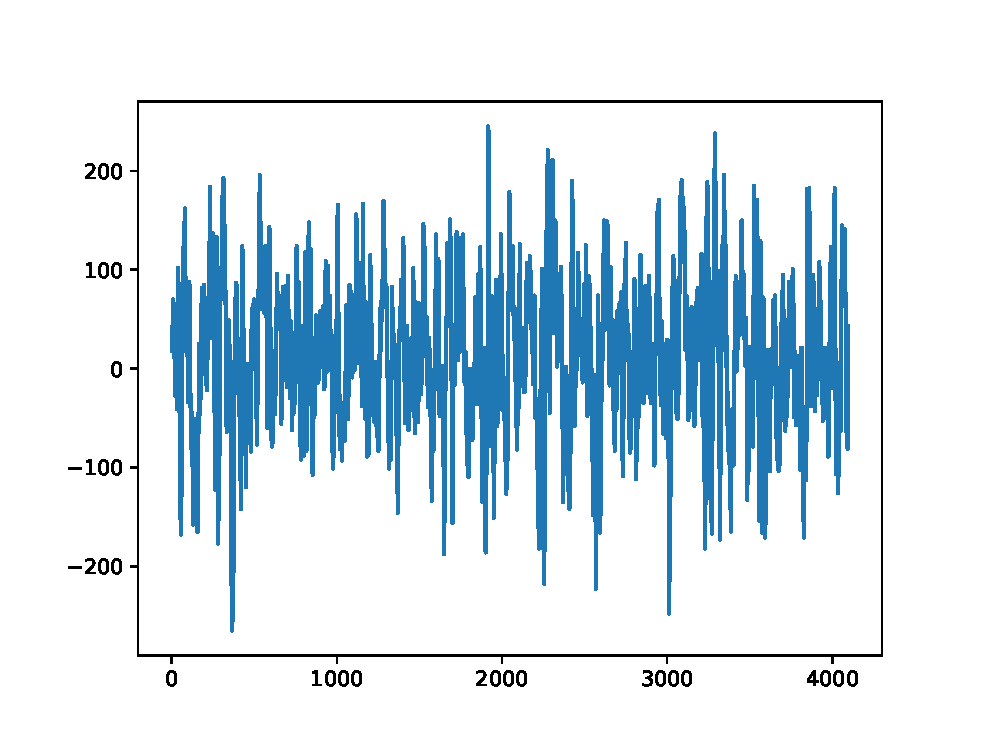
\includegraphics[width=.8\linewidth]{figures/signals/D/F024.eps}
\end{subfigure}
\begin{subfigure}{.25\textwidth}
  \centering
  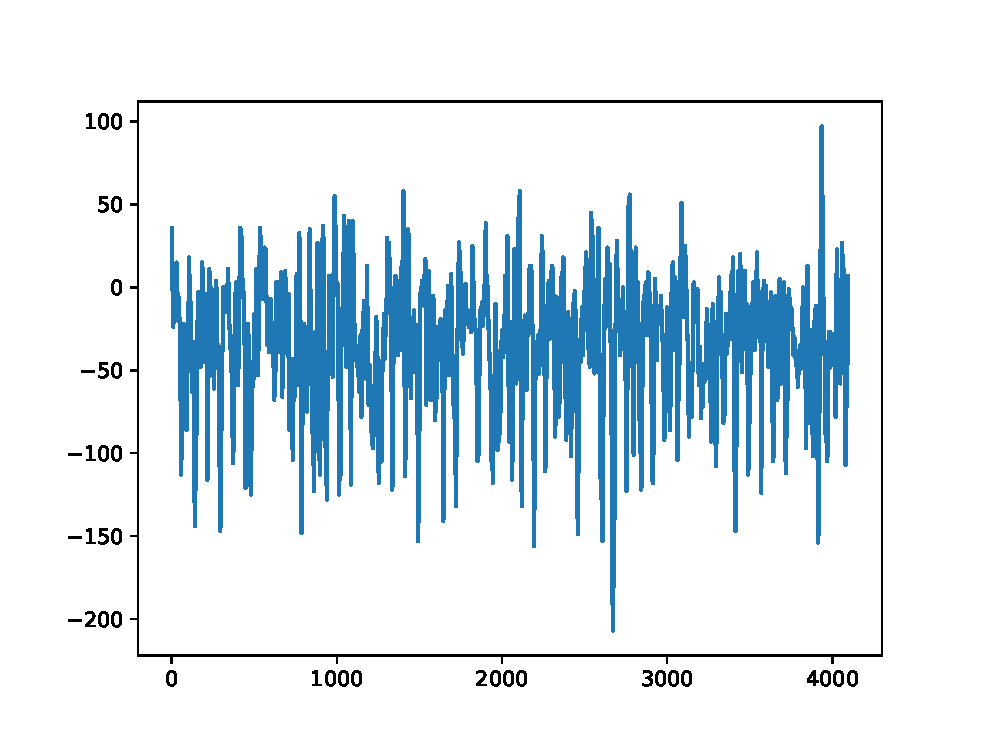
\includegraphics[width=.8\linewidth]{figures/signals/D/F028.eps}
\end{subfigure}%
\begin{subfigure}{.25\textwidth}
  \centering
  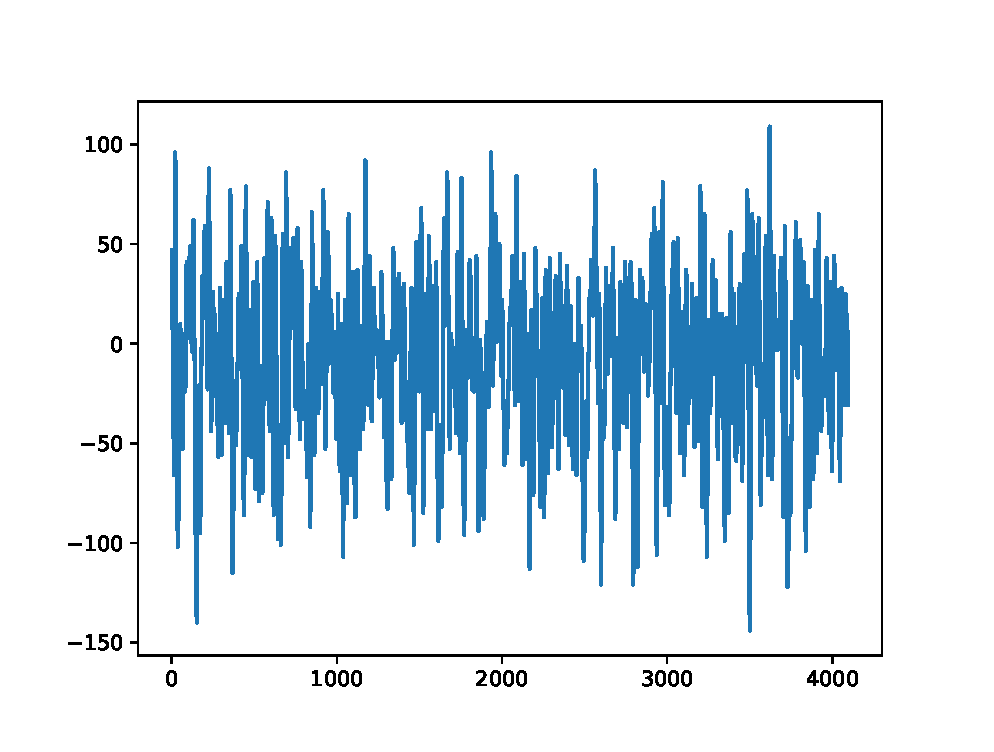
\includegraphics[width=.8\linewidth]{figures/signals/D/F035.eps}
\end{subfigure}

\begin{subfigure}{.25\textwidth}
  \centering
  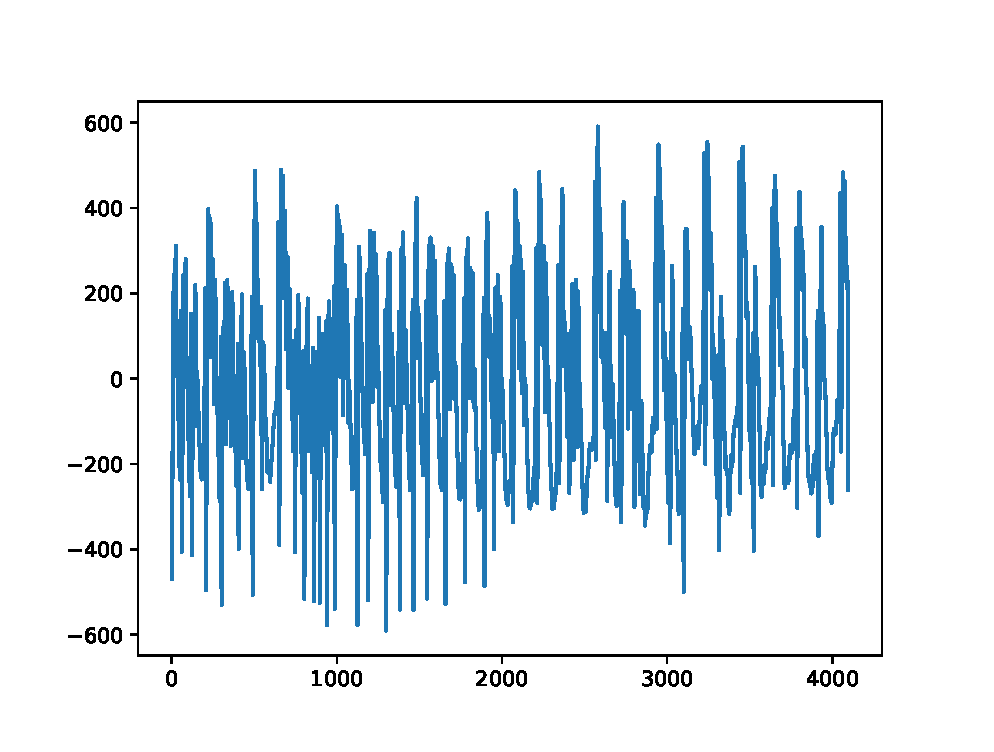
\includegraphics[width=.8\linewidth]{figures/signals/E/S015.eps}
\end{subfigure}%
\begin{subfigure}{.25\textwidth}
  \centering
  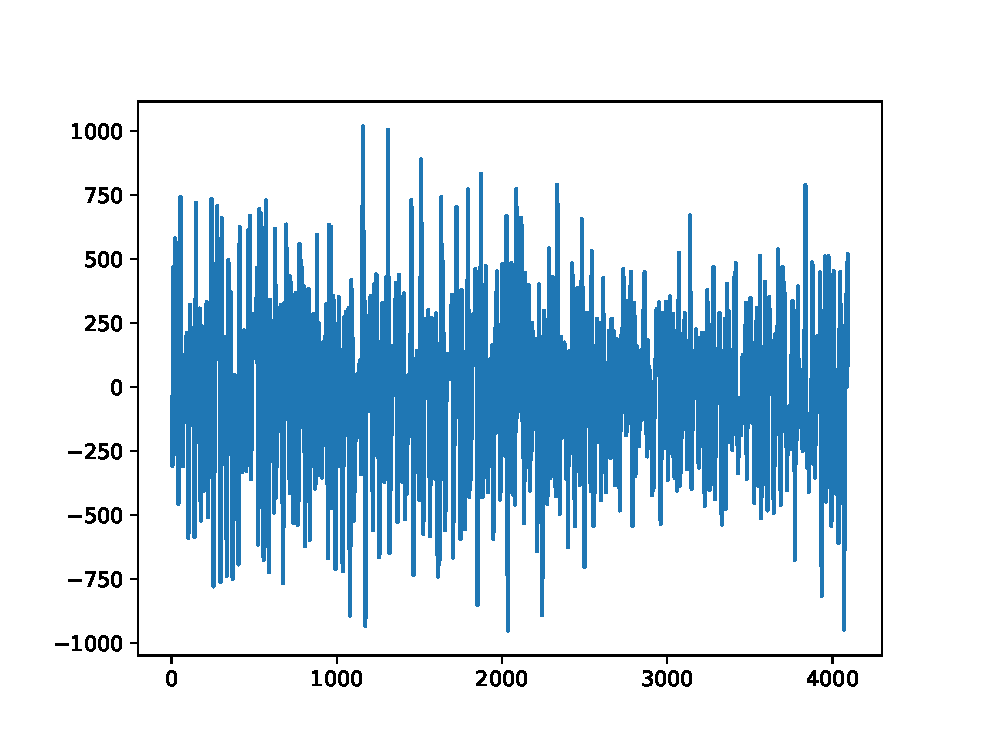
\includegraphics[width=.8\linewidth]{figures/signals/E/S024.eps}
\end{subfigure}
\begin{subfigure}{.25\textwidth}
  \centering
  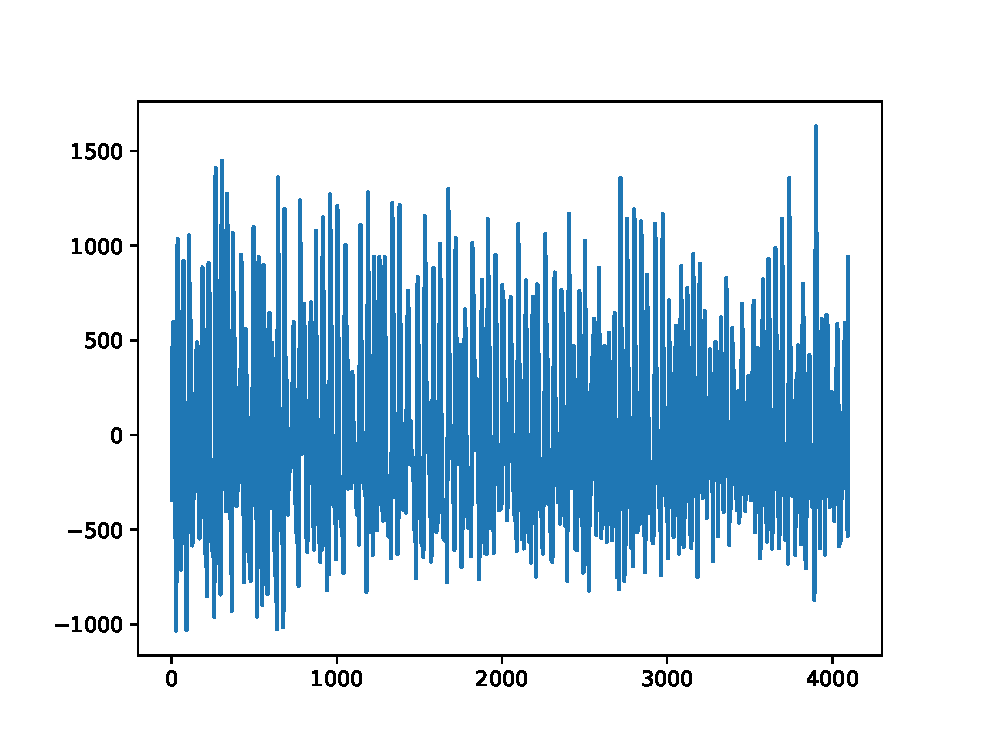
\includegraphics[width=.8\linewidth]{figures/signals/E/S028.eps}
\end{subfigure}%
\begin{subfigure}{.25\textwidth}
  \centering
  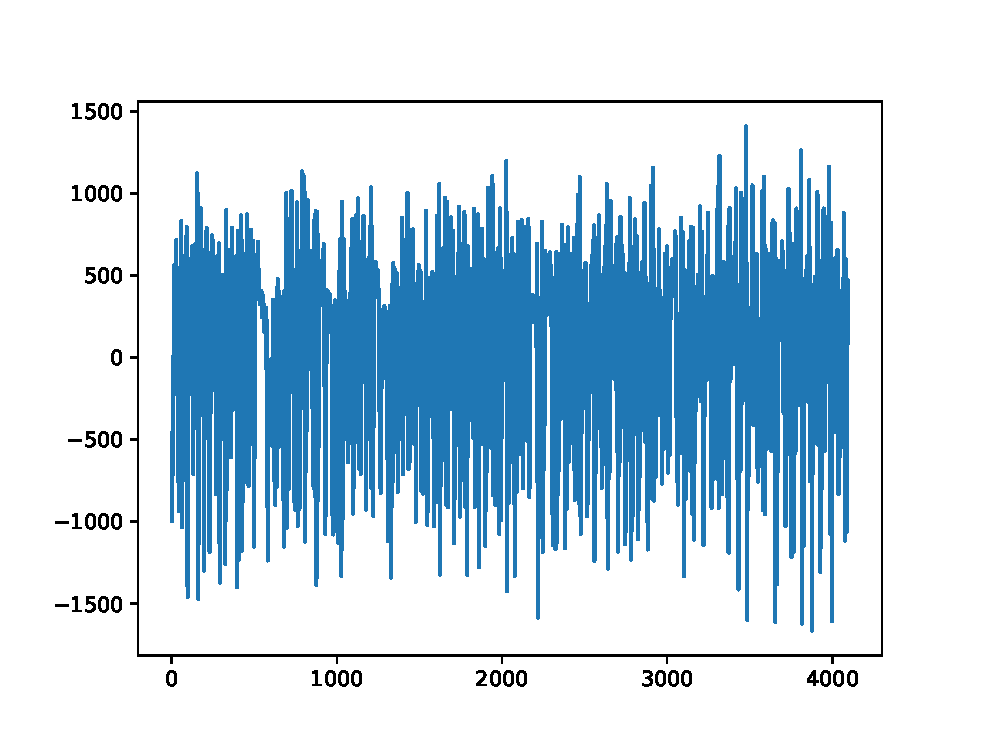
\includegraphics[width=.8\linewidth]{figures/signals/E/S035.eps}
\end{subfigure}
\caption{Images of brain activity signals from patients of classes A (1st row), B(2nd row), C(3rd row), D(4th row) and E(5th row).}
\label{fig:signals}
\end{figure}

\begin{figure}
\begin{subfigure}{.25\textwidth}
  \centering
  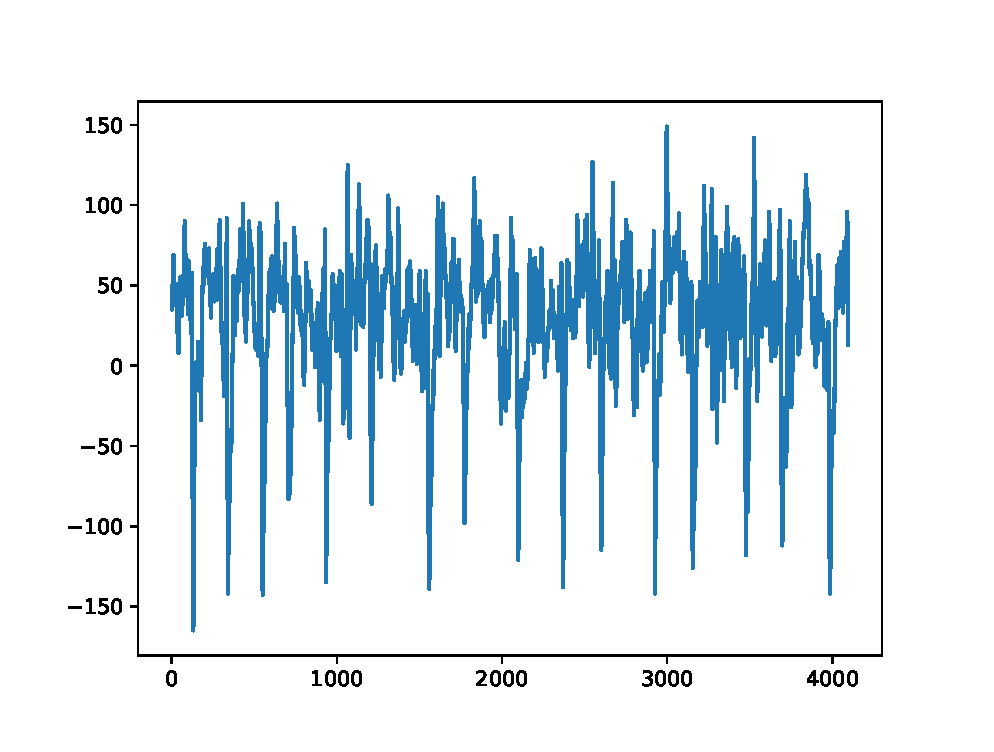
\includegraphics[width=.8\linewidth]{figures/signals/C/N016.eps}
\end{subfigure}%
\begin{subfigure}{.25\textwidth}
  \centering
  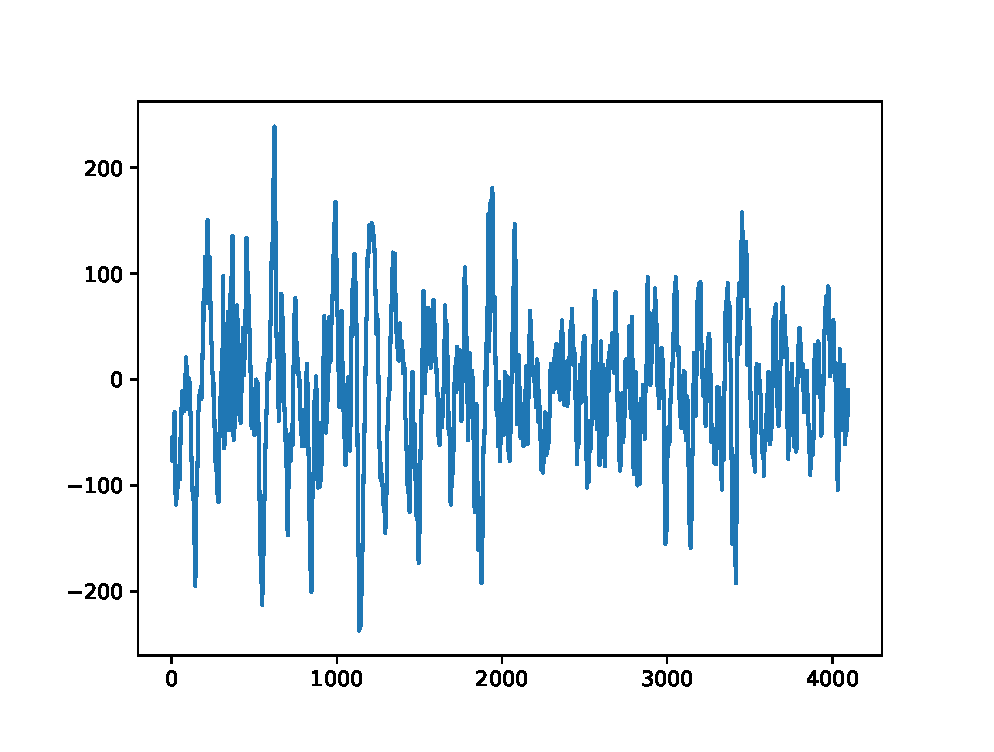
\includegraphics[width=.8\linewidth]{figures/signals/C/N034.eps}
\end{subfigure}
\begin{subfigure}{.25\textwidth}
  \centering
  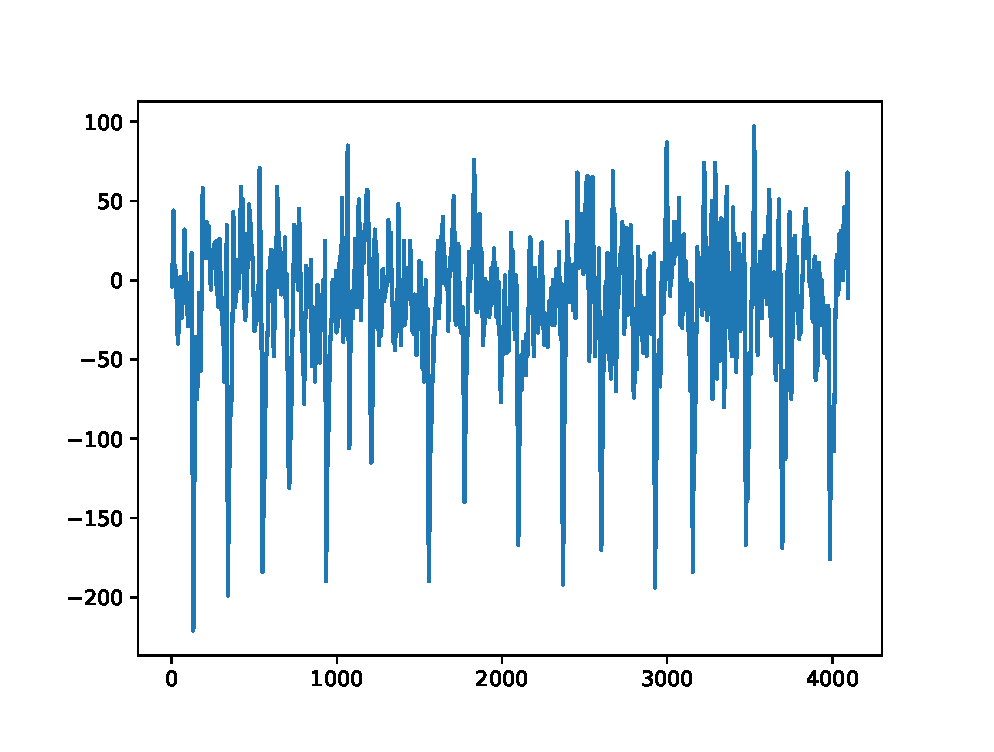
\includegraphics[width=.8\linewidth]{figures/signals/C/N065.eps}
\end{subfigure}%
\begin{subfigure}{.25\textwidth}
  \centering
  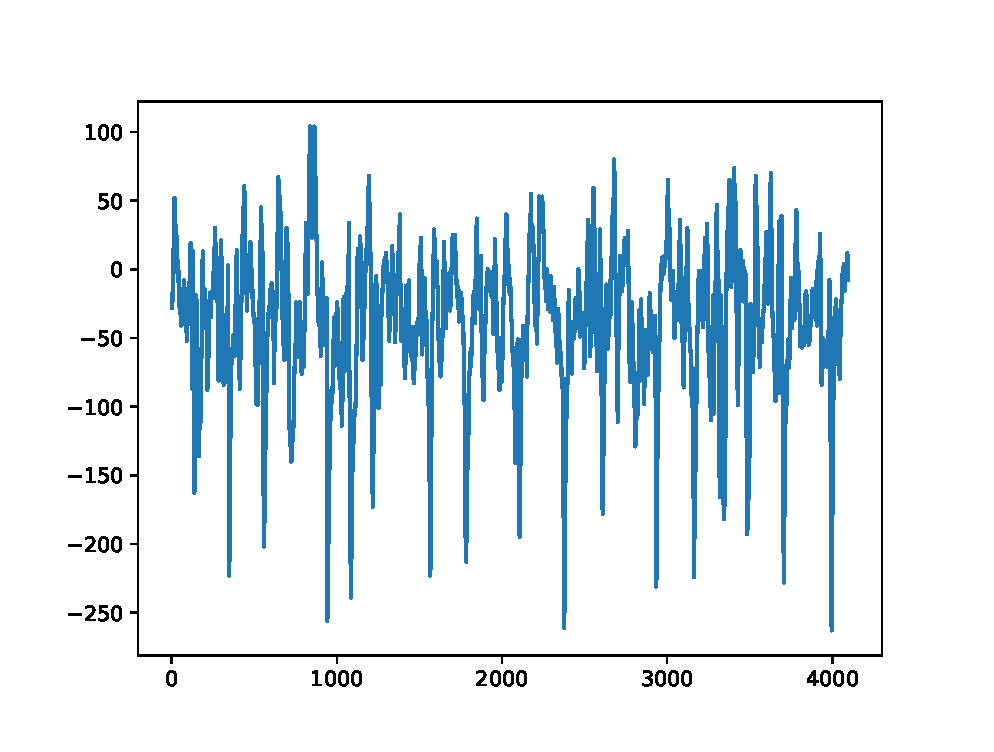
\includegraphics[width=.8\linewidth]{figures/signals/C/N058.eps}
\end{subfigure}

\begin{subfigure}{.25\textwidth}
  \centering
  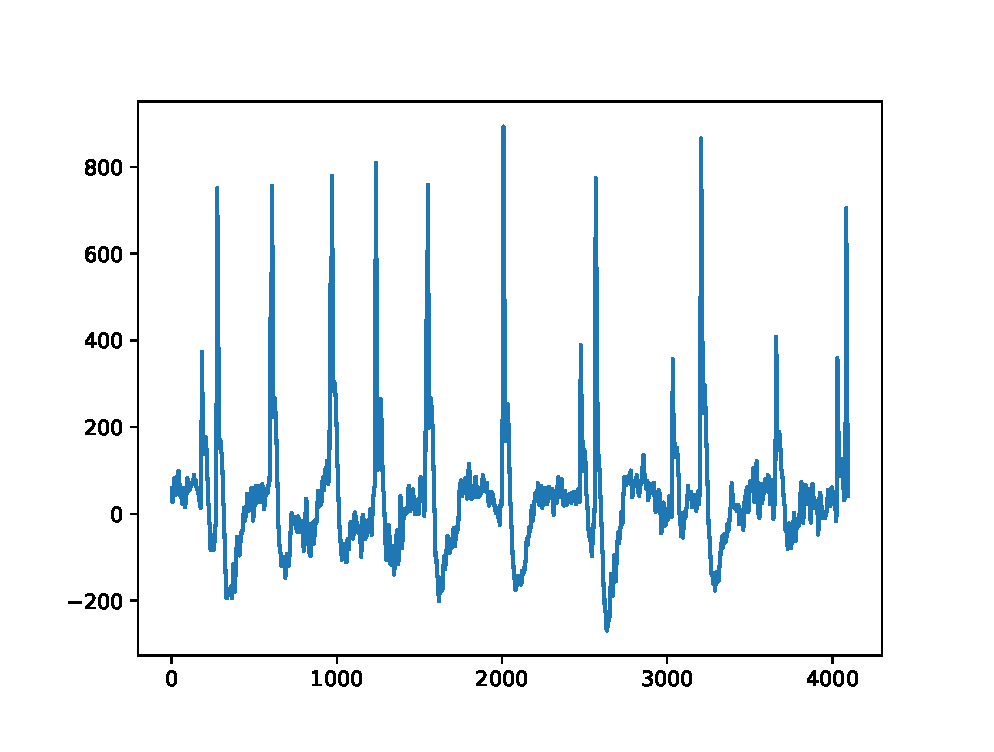
\includegraphics[width=.8\linewidth]{figures/signals/D/F002.eps}
\end{subfigure}%
\begin{subfigure}{.25\textwidth}
  \centering
  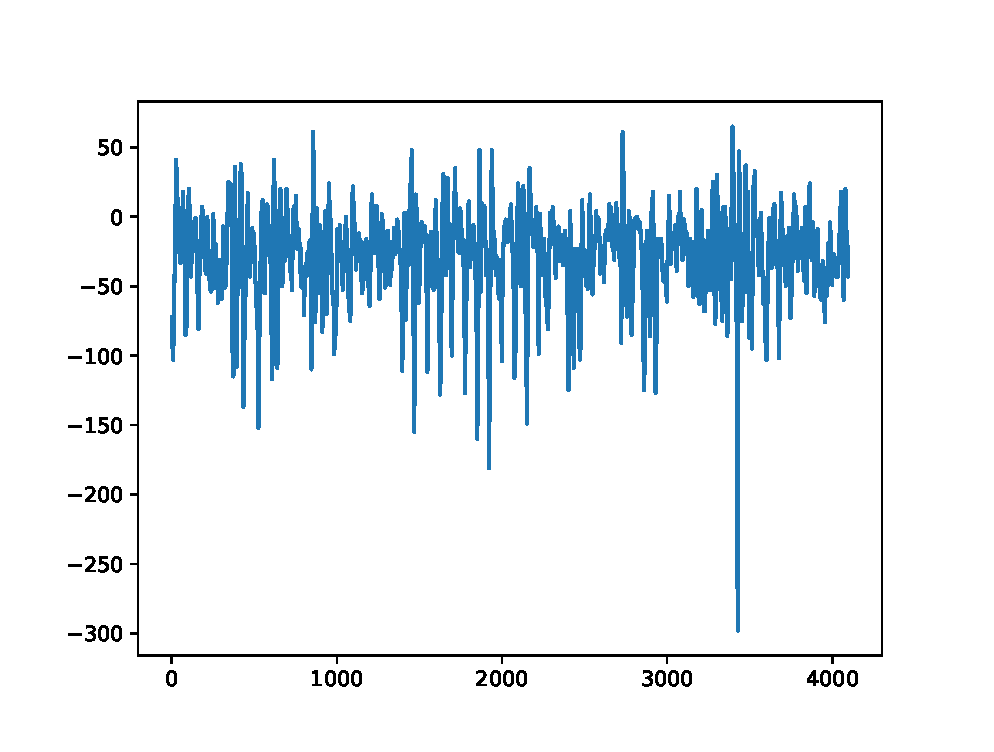
\includegraphics[width=.8\linewidth]{figures/signals/D/F019.eps}
\end{subfigure}
\begin{subfigure}{.25\textwidth}
  \centering
  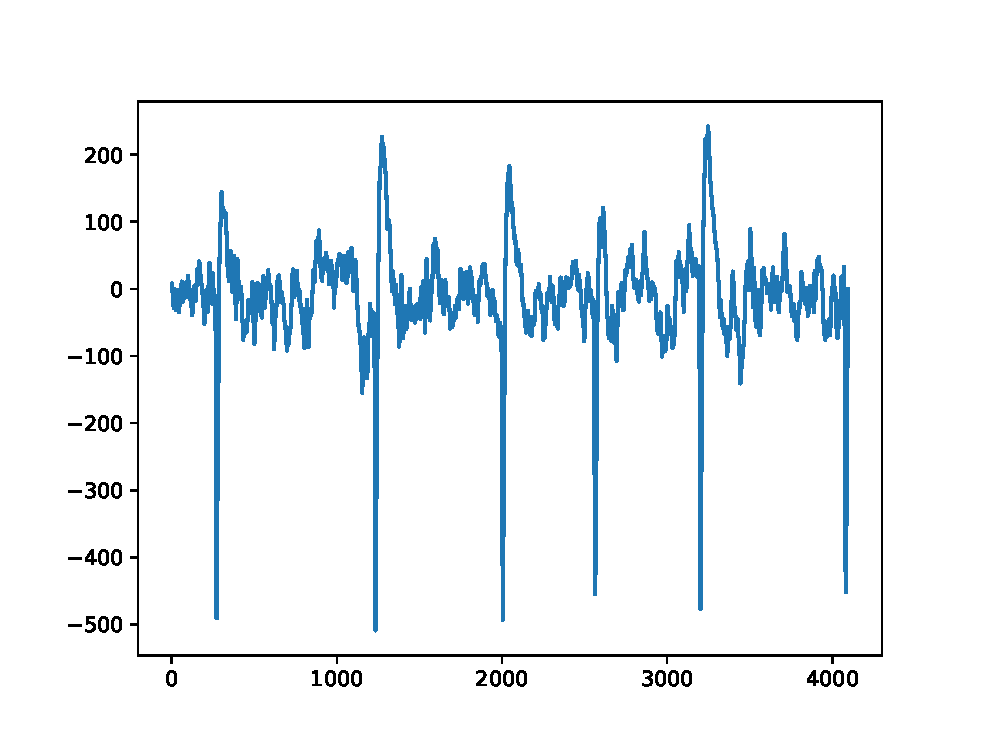
\includegraphics[width=.8\linewidth]{figures/signals/D/F041.eps}
\end{subfigure}%
\begin{subfigure}{.25\textwidth}
  \centering
  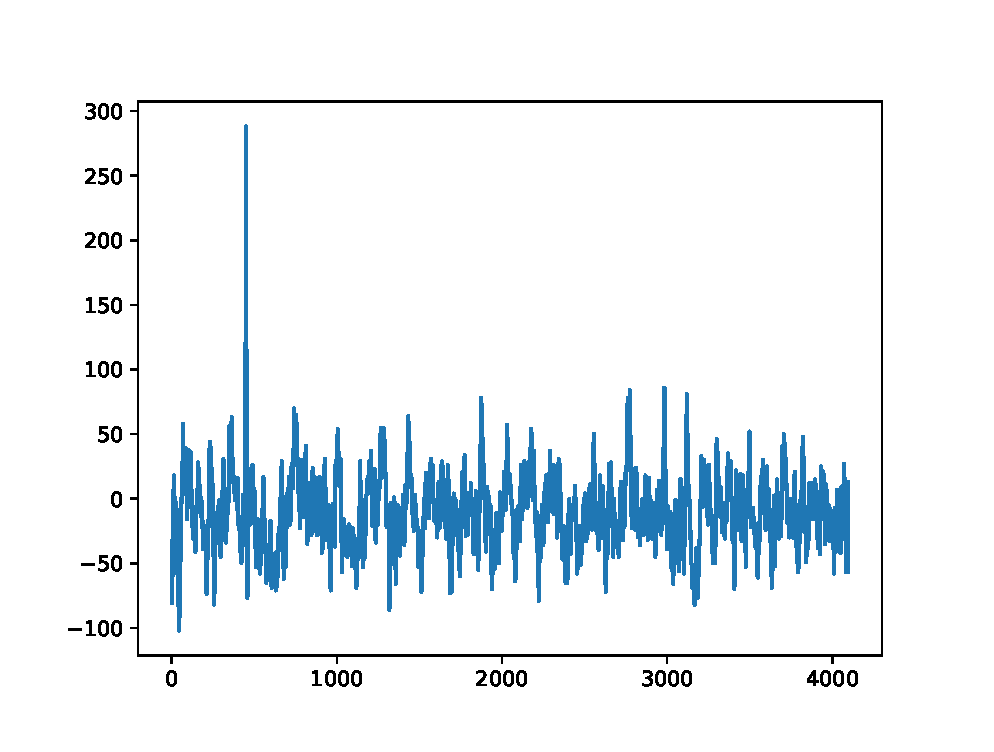
\includegraphics[width=.8\linewidth]{figures/signals/D/F072.eps}
\end{subfigure}

\begin{subfigure}{.25\textwidth}
  \centering
  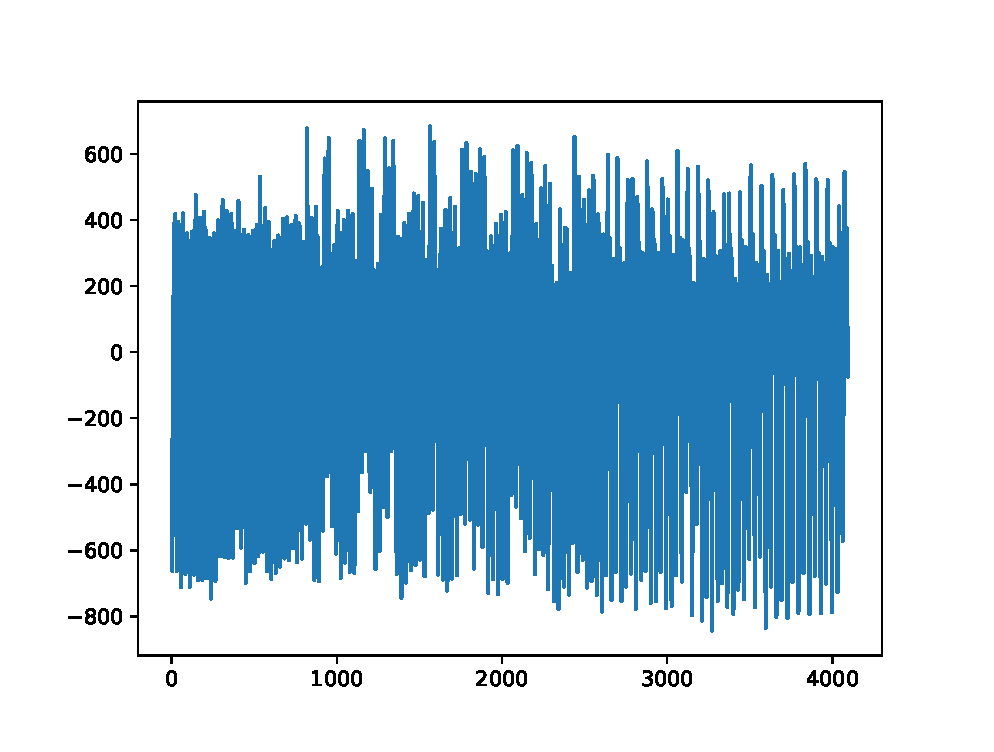
\includegraphics[width=.8\linewidth]{figures/signals/E/S042.eps}
\end{subfigure}%
\begin{subfigure}{.25\textwidth}
  \centering
  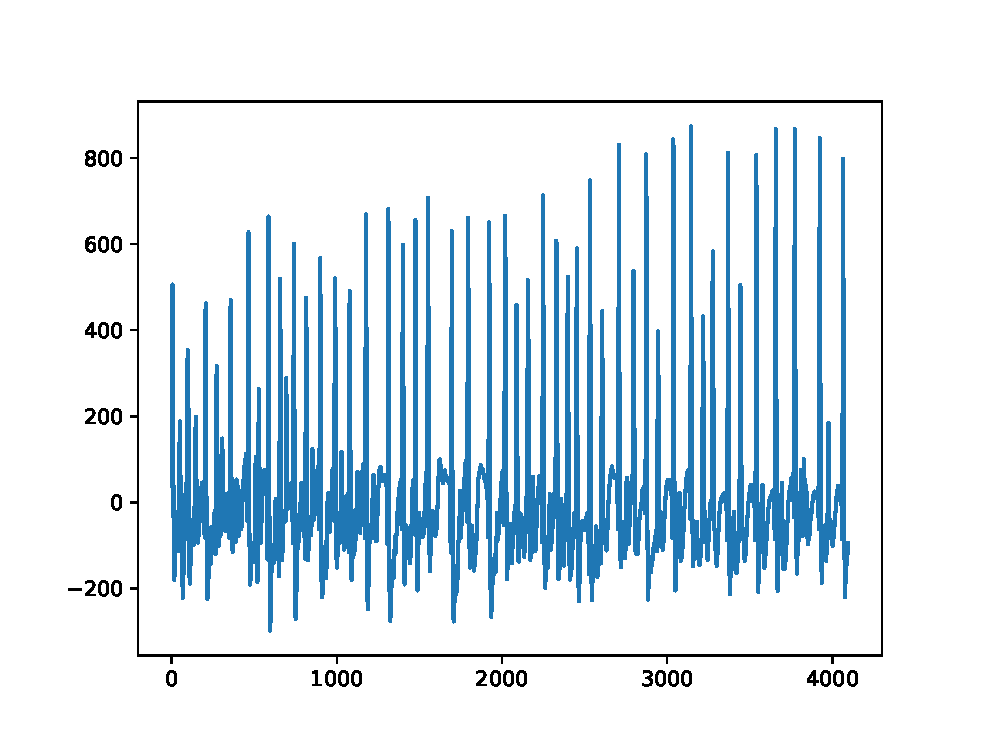
\includegraphics[width=.8\linewidth]{figures/signals/E/S056.eps}
\end{subfigure}
\begin{subfigure}{.25\textwidth}
  \centering
  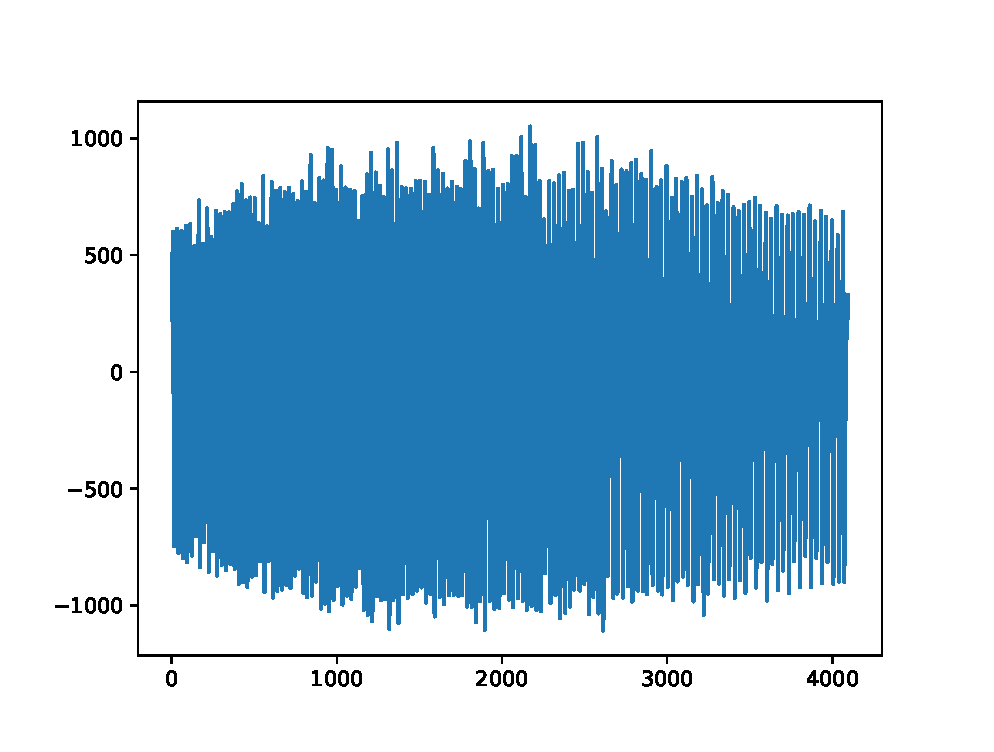
\includegraphics[width=.8\linewidth]{figures/signals/E/S080.eps}
\end{subfigure}%
\begin{subfigure}{.25\textwidth}
  \centering
  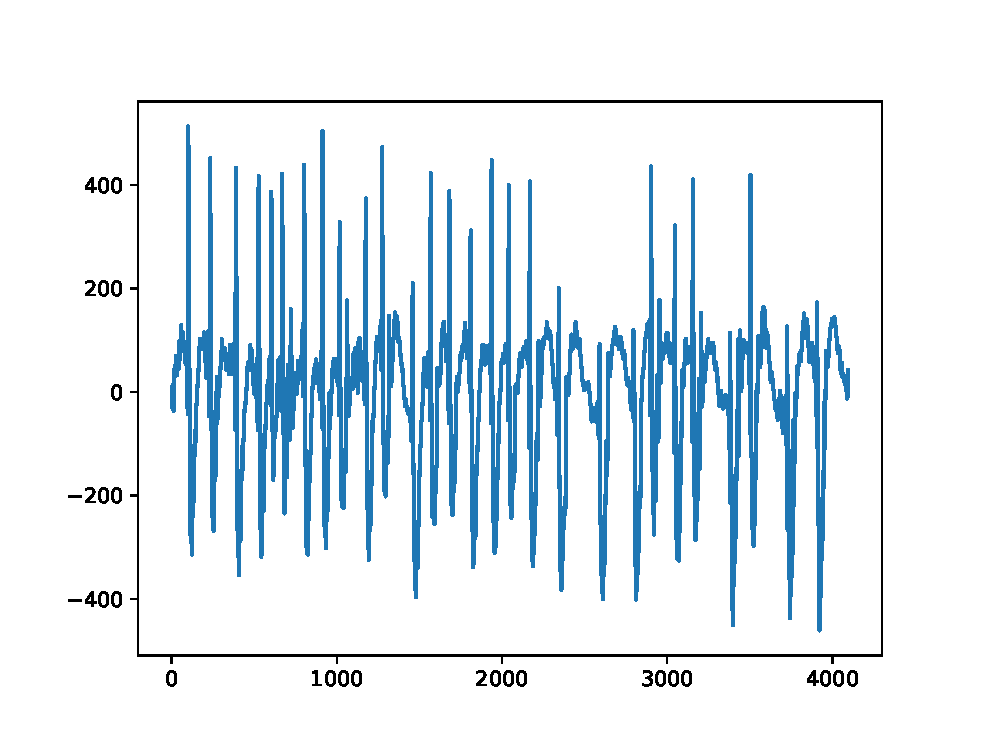
\includegraphics[width=.8\linewidth]{figures/signals/E/S084.eps}
\end{subfigure}
\caption{Some distinguished signals from patients of classes C (1st row), D(2nd row), E(3rd row).}
\label{fig:odd_signals}
\end{figure}

Figure~\ref{fig:statistics} shows the chart of common statistics of signal values within each class, and the detailed numbers are shown in Table~\ref{tab:statistics}. The data points of class E, the category of patients in their seizure-active periods, have the smallest average value ($-4.74$) but spread the most among the classes with standard deviation $341.15$ (more than the total standard deviation of all the other classes). The four classes A, B, C and D appear to have similar percentiles of $25\%$, $50\%$ and $75\%$; however, data points in class D appear to spread wider than those in the other three classes. The ranges of minimal and maximal values are perhaps the most visible distinction between the two sets $A \cup B$ and $C \cup D$.

\begin{figure}
\begin{subfigure}{.5\textwidth}
  \centering
  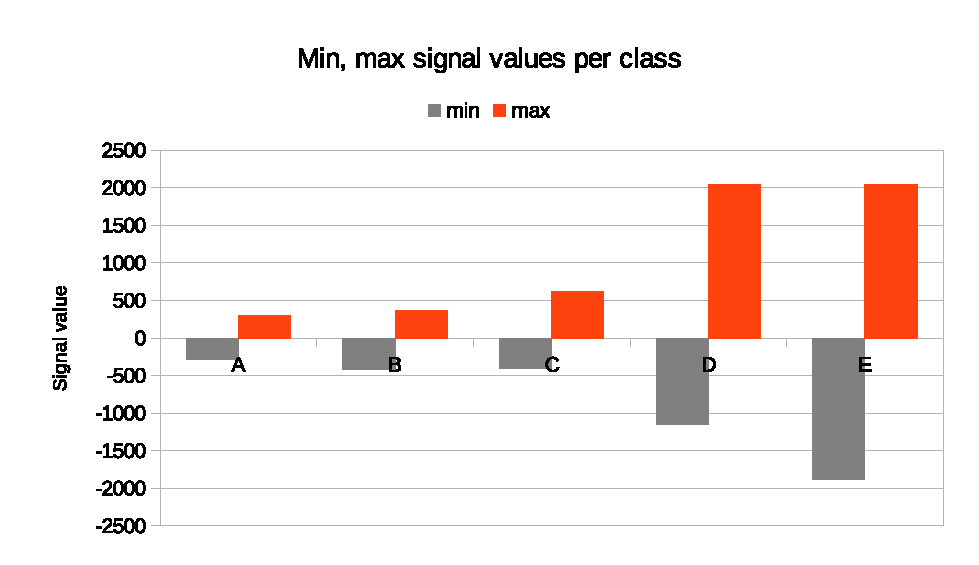
\includegraphics[width=.8\linewidth]{figures/minmax.eps}
\end{subfigure}%
\begin{subfigure}{.5\textwidth}
  \centering
  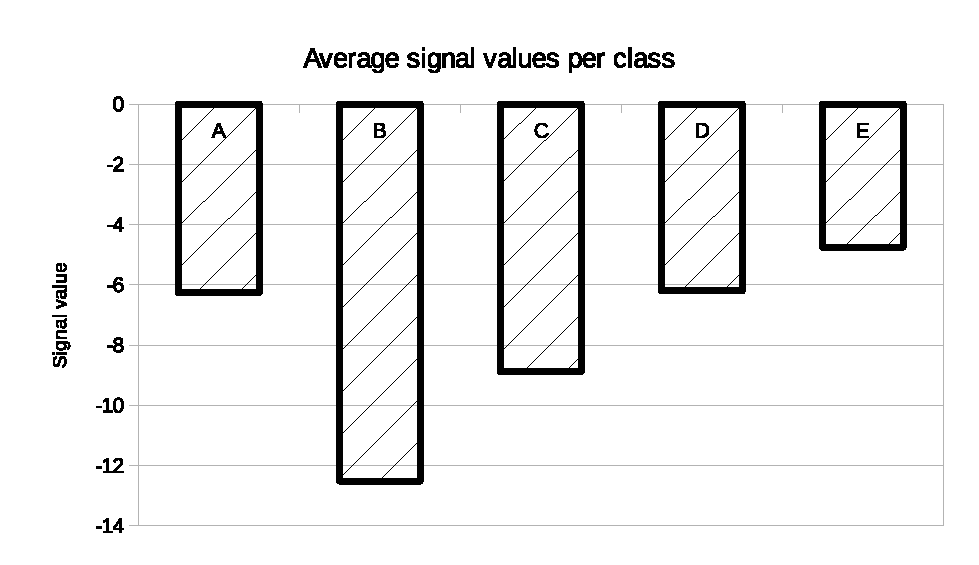
\includegraphics[width=.8\linewidth]{figures/mean.eps}
\end{subfigure}

\begin{subfigure}{.5\textwidth}
  \centering
  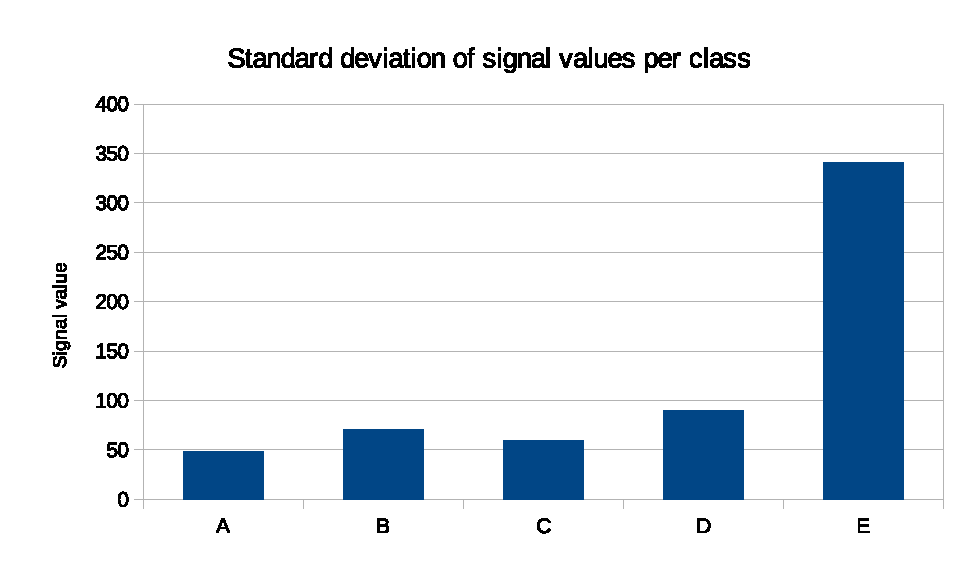
\includegraphics[width=.8\linewidth]{figures/std.eps}
\end{subfigure}%
\begin{subfigure}{.5\textwidth}
  \centering
  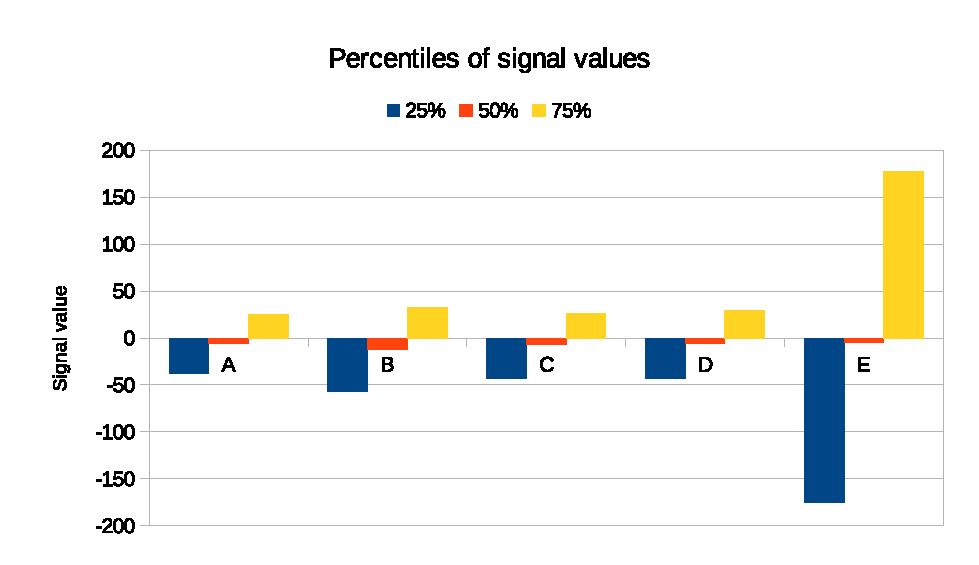
\includegraphics[width=.8\linewidth]{figures/percentiles.eps}
\end{subfigure}
\caption{Some statistics of the data set per class: min, max (top left), mean (top right), standard deviation (bottom left) and percentiles (bottom right).}
\label{fig:statistics}
\end{figure}

\begin{table}
\begin{center}
\begin{tabular}{|l||c|c|c|c|c|c|c|}
\hline
Class & Min & Max & Mean & Stddev & $25\%$ & $50\%$ & $75\%$ \\ \hline \hline
$A$ & -288 & 294 & -6.26 & 48.33 & -38 & -6 & 25 \\ \hline
$B$ & -424 & 360 & -12.51 & 70.68 & -57 & -12 &	32 \\ \hline
$C$ & -412 & 623 & -8.88 & 59.38 & -43 & -7 & 26 \\ \hline
$D$ & -1147 & 2047 & -6.20 & 90.34 & -43 & -6 & 29 \\ \hline
$E$ & -1885 & 2047 & -4.74 & 341.15 & -175 & -5 & 177 \\ \hline
\end{tabular}
\caption{Statistics of the data set per class.}
\label{tab:statistics}
\end{center}
\end{table}


\subsection{Algorithms and Techniques}
\label{sec:solution}

\noindent
As mentioned earlier, much work has been done on this data set that focused on extracting hand-crafted features to be used for classifying the segments into volunteer target classes (\cite{nigam2004neural}, ~\cite{guler2005recurrent}, ~\cite{kannathal2005entropies}). Since the ability to automatically learn features and representations is a key benefit of machine learning, a reasonable question is whether one could automatically learn features from the EEG signals in this domain for classification purposes, and if so then which algorithm could be used effectively.

Deep architectures of neural networks have been successful recently in many machine learning applications, and part of their success is due to their ability to learn high-level features. On the other hand, training deep networks is costly, and one way to tackle this challenge is to initialize their parameters with values obtained from pretraining some types of networks. Two types of such networks have been widely used: restricted Boltzmann machines~\cite{hinton2006reducing} and autoencoders\cite{bengio2007greedy}. For EEG signal domains, previous work such as Wulsin et al.~\cite{wulsin2011modeling} pretrained restricted Boltzmann machines for feature learning and classification, and although Bengio et al.~\cite{bengio2007greedy} showed that autoencoders worked equally well as restricted Boltzmann machines, there were no previous work, to the best of my knowledge, which used autoencoders for learning representations and classification in the epileptic seisure domain~\cite{andrzejak2001indications} of interest.

The proposed approach therefore is to train autoencoders for extracting representations of the input signals, and then ultilize the pretrained autoencoders to form a deep neural network for the classification task at hand. The architecture of multi-layer feed-forward neural networks was chosen as (1) it can nicely incorporate the encoding parts of the pretrained autoencoders, and (2) it allows for \textit{fine-tuning} the pretrained parameters for classifying the specific target classes, a technique that usually help improve the performance of deep neural networks.

\subsubsection{Training autoencoders}
\noindent
A \textit{traditional autoencoder} (\cite{bengio2007greedy}, \cite{vincent2010stacked}) is a fully connected feed-forward neural network which consists of an input layer, one hidden layer and an output layer such that the input and output layers have the same number of neurons. The computation performed by the hidden layer, specified by a weight matrix $\myvec{W}$, bias vector $\myvec{b}$ and nonlinear activation function $s$, acts as an \textit{encoder} that maps an input vector $\myvec{x}$ to a representation $f_{\theta}(\myvec{x})$ defined as follows:

\[f_{\theta}(\myvec{x}) = s(\myvec{W}\myvec{x} + \myvec{b}).\]

The parameter set $\theta=(\myvec{W}, \myvec{b})$ is part of what to be adjusted. The encoding $f_{\theta}(\myvec{x})$ is then mapped back to vector $\myvec{z}$ in the same space with $\myvec{x}$ through the computation of the output layer, representing the \textit{decoder} part of the autoencoder:

\[\myvec{z} = g_{\theta'}(f_{\theta}(\myvec{x})),\]

\noindent
where $g_{\theta'}$ can be either a linear or a non-linear function whose parameter $\theta'$ is the other part of what to be learned. With real-valued input signals $\myvec{x}$, the output $\myvec{z}$ in general is interpreted not as the exact reconstruction of $\myvec{x}$ but the mean of a distribution $P(\myvec{x}|\myvec{z})$. Squared error function between $\myvec{x}$ and $\myvec{z}$, and thus the objective function

\[L(X) = \frac{1}{N}\sum_{i=1}^{N}(\myvec{x_i} - \myvec{z_i})^2,\]
\noindent
is to be optimized during the training of the autoencoders. As suggested in~\cite{vincent2010stacked}, affine mapping is to be used for this type of real-valued inputs and error function; in other words, $g_{\theta'}(\myvec{y}) = \myvec{W}' \myvec{y} + \myvec{b}'$ and $\theta'=(\myvec{W}', \myvec{b}')$.

In order for autoencoders not to produce trivial encoding and decoding functions (e.g., to avoid the identity function from input $\myvec{x}$ to itself), certain types of constraints need to be imposed. In traditional autoencoder, a constraint could be that the number of neurons of the hidden layer is smaller than the dimension of the inputs $\myvec{x}$. In so-called \textit{denoising autoencoders}~\cite{vincent2010stacked}, the inputs are made ``dirty'' before being fed into the encoder---by attempting to reconstruct the original input from its corrupted version, denoising autoencoders might learn representations that are more essential to the inputs. In this work, the input signals are made corrupted using one of the following two ways:
\begin{itemize}
\item Adding into the inputs random noises generated by a Gaussian distribution with zero mean and $\sigma$ standard deviation $N(0,\sigma^2)$.
\item Disable a random number of neurons at the input layer of the autoencoders, which can be implemented using dropout techniques~\cite{srivastava2014dropout} with dropout rate denoted by $\rho$ ($0 < \rho < 1$).
\end{itemize}

\subsubsection{Stacking up autoencoders}
\noindent
The idea of reconstructing the inputs using autoencoders can be applied to map the orginal input into a highly non-linear representations. Specifically, the process starts by training the first autoencoder, defined by encoding and decoding functions $f^{(1)}_{\theta_1}$ and $g^{(1)}_{\theta'_1}$, to reconstruct input vector $\myvec{x}$. The representation of $\myvec{x}$ is then obtained by applying the learned encoding function to $\myvec{x}$, i.e. $f^{(1)}_{\theta_1}(\myvec{x})$. For each index $i \geq 1$, the representation $f^{(i)}_{\theta_i}(\myvec{x})$ produced from training the $i$th autoencoder becomes the input to the next $(i+1)$-th autoencoder, which is then trained to adjust its parameter $\theta_{i+1}$ and  $\theta'_{i+1}$ of the encoding and decoding functions $f^{(i+1)}_{\theta_{i+1}}$ and $g^{(i+1)}_{\theta'_{i+1}}$, respectively. From the resulting sequence of trained encoders $\langle f^{(1)}_{\theta_1}, f^{(2)}_{\theta_2}, ..., f^{(k)}_{\theta_k} \rangle$, the original input $\myvec{x}$ can then be mapped into the representation computed as $f^{(k)}_{\theta_k}(f^{(k-1)}_{\theta_{k-1}}(...(f^{(1)}_{\theta_1}(\myvec{x}))))$.

More importantly, a multi-layer feed-forward neural network can be built based on the sequence of trained autoencoders for our classification task. The network consists of the following components:
\begin{itemize}
\item an input layer of $M$ neurons, where $M$ is the number of dimension of the input vectors, that accepts input signals $\myvec{x}_i \in X$;
\item a sequence of $k$ hidden layers where the $i$th layer ($i \geq 1$) is the hidden layer of the $i$-th pretrained autoencoder, i.e. \textit{the weights and biases are initialized with the pretrained values};
\item a softmax output layer with three neurons for the three target classes \textit{whose weights and biases are randomly initialized}.
\end{itemize}

The above network can be used in two ways. In the first approach, the weights and biases of all the hidden layers are freezed, and the parameters of the output layer are to be trained subject to the reconstruction error defined on the training set $X$; in other words, the representations $f^{(k)}_{\theta_k}(f^{(k-1)}_{\theta_{k-1}}(...(f^{(1)}_{\theta_1}(\myvec{x}))))$ are used directly as the inputs to the output layer whose parameters are the only ones to be adjusted by the network during learning. The second approach, which results in better accuracy, is fine-tuning the entire network's parameters for the classification task. By starting from the pretrained weights and biases in the hidden layers, we can train an instance of the above networks with competitive accuracy performance, compared to other methods solving this problem using hand-crafted features.

\subsection{Benchmark}
\noindent
The main purpose of this work is to explore the benefit of using pretrained autoencoders to train a multi-layer feed-forward neural network for the classification task at hand. Secion~\ref{sec:results} presents several results between different design choices and network configurations. For external comparisons, previous work has been developed for the classification problem on the same data set~\cite{andrzejak2001indications}; the main contribution of most of these work, however, were on designing various hand-crafted features for the EEG signals. They might also be different from each other in the target classes of interest. As examples, Nigam and Graupe~\cite{nigam2004neural} used two features based on the spike information of the signals for further learning and detecting patients in set $E$ (thus, binary classification problem). Kabir et al.~\cite{kabir2016epileptic} extracted statistical features based on ``optimum allocation technique'' to be used with logistic model trees for classifying volunteers into the three classes that are of interest of this project. Guler et al.~\cite{guler2005recurrent} employed Lyapunov exponents based features for classification using recurrent neural networks where the target classes are three sets $A$, $D$ and $E$. On another data set, Wulsin et al.~\cite{wulsin2011modeling} learned features of second-long segments of EEG signals using Deep Belief Networks~\cite{hinton2006reducing} and classified them into ``clinically significant'' EEG classes. To the best of my knowledge, there was no previous work reporting the results of using autoencoders for the data set that this project is interested in.

The proposed method by Kabir et al.~\cite{kabir2016epileptic} on the data set of interest in this project outperforms many the state-of-the-art approaches using the same data set; among many other measures, the total accuracy of their approach was $95.3\%$. Since its target classes are the same with those of interest in this project, and their work represents a class of work using hand-crafted features, it is reasonable to use the performance of their work as the baseline for the approach to be explored in this project. The hypothesis is that by using autoencoders, it is possible to learn a set of features automatically for classifying EEG signals with comparable results.

\section{Methodology}
\subsection{Data Preprocessing}

The data set~\cite{andrzejak2001indications} contains 100 channels (vectors of micro-voltage values) for each of the five sets of volunteers. Each channel is a vector of 4097 values that are EEG signals recorded in $23.6$ seconds. The data set is then preprocessed as follows.
\begin{itemize}
\item Each channel is divided into 23 one-second segments with equal length, each contains 178 values. These segments are marked with the target value $0$, $1$ or $2$ for the classes $A + B$, $C + D$ and $E$ of the original channel.
\item The resulting set of segments are splitted into three separate sets for training ($60\%$), validation ($20\%$) and testing ($20\%$) (using StratifiedShuffleSplit function from Scikit-Learn).
\item The resulting set of segments in the training set are then normalized so that the values of EEG signals are in between $[-1,1]$. The internal state of the scaler (which contains for example the min and max signal values of the training set) is used to scale the other two sets into the same interval.
\end{itemize}

\subsection{Implementation}

\noindent
The approach proposed in this project was implemented in Python 3 using TensorFlow library, and its source code could be found at the following link:
\begin{center}
\href{https://github.com/natuan/ml\_nano\_capstone.git}{\textit{https://github.com/natuan/ml\_nano\_capstone.git}}.
\end{center}

In the following, I discuss at high level the key components of the implementation of autoencoders, the derived feed-forward neural network, and the elements that support for their training and testing.

\subsubsection{Autoencoders}
\noindent
The autoencoders were implemented in the class \texttt{UnitAutoencoder} inside folder \textit{src/StackedAutoencoders.py}. Figure~\ref{fig:autoencoders} shows the conceptual image of the two types of autoencoders, optionally with dropout applied to the hidden layers for dealing with overfitting. In TensorFlow, the key elements of the autoencoders can be implemented roughly as follows.

\begin{figure}
  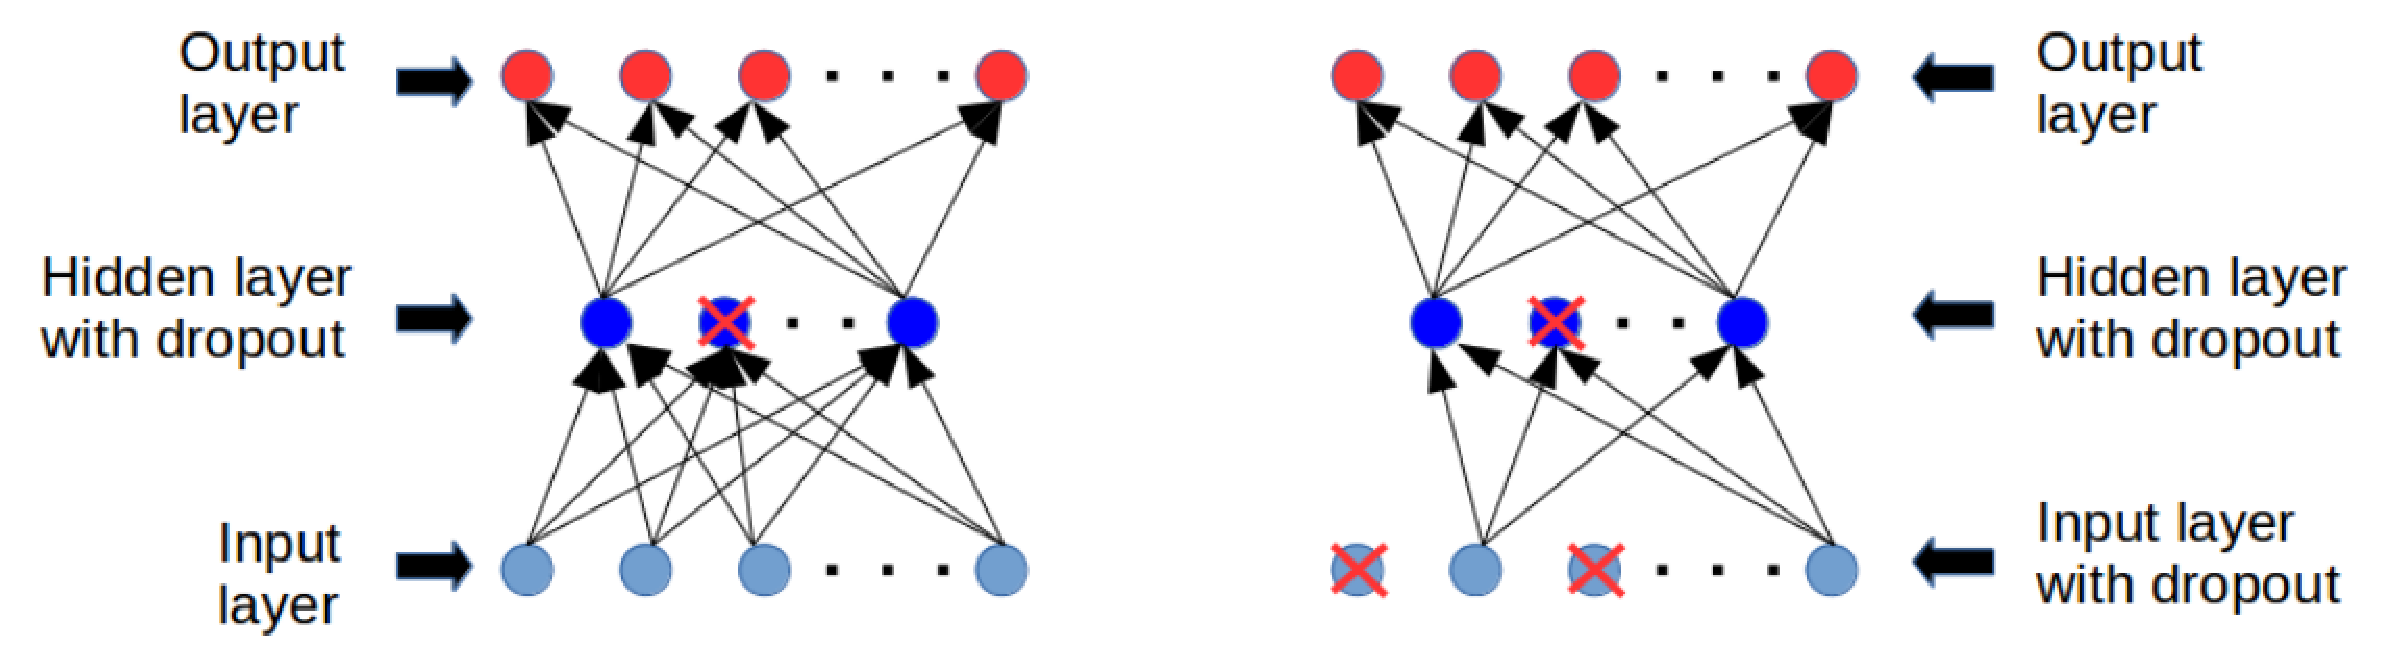
\includegraphics[width=0.9\linewidth]{figures/autoencoders.eps}
  \caption{Traditional (left) and denoising (right) autoencoders with an input layer, a hidden layer and an output layer. Dropout technique is applied to hidden layers in the two types of autoencoder for dealing with overfitting, and to the input layer also for corrupting the input vectors.}
  \label{fig:autoencoders}
\end{figure}

\textit{Input tensors}: the input vectors of size \texttt{n\_inputs} are placed into a ``place holder''\footnote{Here \texttt{tf} stands for the imported module tensorflow.}:
\begin{verbatim}
  X = tf.placeholder(tf.float32,
                     shape=[None, n_inputs],
                     name='X'),
\end{verbatim}
\noindent
whose value will be assigned at run-time. To facilitate the use of dropout, which takes effect only during training, one needs also define a boolean tensor as another input of the network indicating the training/test mode:
\begin{verbatim}
  training = tf.placeholder_with_default(False, 
                                         shape=(), 
                                         name='training').
\end{verbatim}

\textit{Input layer}: the input layer of the traditional autoencoders is specified simply with the tensor $X$. When dropout is used to corrupt the inputs for denoising autoencoders, the dropout layer construct in TensorFlow, \texttt{tf.layers.dropout}, can be used on top of the original input if the \texttt{training} is set to be \texttt{True}:
\begin{verbatim}
  X_noisy = tf.layers.dropout(X, input_dropout_rate, 
                              training=training),
\end{verbatim}
\noindent
where the second parameter specifies the dropout rate. Alternatively, Gaussian noises, implemented using \texttt{tf.random\_normal}, can be used to corrupt the inputs if the network is in training mode:
\begin{verbatim}
  X_noisy = tf.cond(training,
                    lambda: X + tf.random_normal(tf.shape(self.X), 
                                                 stddev = noise_stddev),
                    lambda: X).
\end{verbatim}

\textit{Hidden layer}: The construct \texttt{tf.layers.dense} can be used to construct the dense hidden layer of \texttt{n\_neurons} neurons right after \texttt{X\_noisy} as follows:
\begin{verbatim}
  dense_hidden = tf.layers.dense(X_noisy, n_neurons, 
                                 activation=hidden_activation,
                                 ...),
\end{verbatim}
\noindent
where \texttt{hidden\_activation} specifies the activation function used for the neurons. (Unused arguments were omitted to simplify discussion.) A dropout layer could then be put on top of the hidden layer for dealing with the overfitting issue:
\begin{verbatim}
  hidden = tf.layers.dropout(dense_hidden, 
                             hidden_dropout_rate,
                             training=training),
\end{verbatim}
where \texttt{hidden\_dropout\_rate} defines the dropout rate for the hidden layer.

\textit{Output layer}: the output layer of \texttt{n\_inputs}, the same size with the input layer, can be implemented using \texttt{tf.layers.dense}, right after the layer \texttt{hidden} above:
\begin{verbatim}
  outputs = tf.layers.dense(hidden, 
                            n_inputs, 
                            activation=output_activation,
                            ...).
\end{verbatim}
The \texttt{output\_activation} can be used to customize the activation function for the output layer; as mentioned earlier an affine mapping should be used given the real-valued inputs and the squared reconstruction error function.

\textit{Reconstruction error}: in order to extract representations of the inputs, the autoencoder is trained to minimize the difference between its outputs and the original inputs. The reconstruction error is defined using the squared-error loss:
\begin{verbatim}
  reconstruction_loss = tf.reduce_mean(tf.square(outputs - X)).
\end{verbatim}

\textit{Training operator}: To train the network, a training operator first needs to be defined to optimize the above reconstruction loss:
\begin{verbatim}
  training_op = optimizer.minimize(reconstruction_loss).
\end{verbatim}

Each step of the training is performed by running the training operator within a TensorFlow session \texttt{sess}, feeding the network with a current batch \texttt{X\_batch} and the \texttt{True} value for input tensors \texttt{X} and \texttt{training}, respectively:
\begin{verbatim}
  sess.run(training_op, feed_dict={X: X_batch, 
                                   training: True}).
\end{verbatim}

\subsubsection{Building a feed-forward neural network from pretrained autoencoders}

\noindent
Recall that the computation of hidden layers in the autoencoders is intended to act as their encoder, and that of the output layers as their decoders. By putting together the encoding parts of a sequence of autoencoders, one can build an expressive encoder that consists of a multiple layers of neurons. The feed-forward network for the problem of interest is largely built based upon those stacked up pretrained encoders, together with a softmax output layer for the classification purpose. While the autoencoders are trained in an unsupervised fashion (their inputs are also their expected outputs), the network is designed for supervised learning with predefined target classes. The network's tensor inputs, therefore, must include a tensor \texttt{y} representing the target class, in addition to the tensor representing the input vectors \texttt{X} and the training/testing mode \texttt{training}:
\begin{verbatim}
  y = tf.placeholder(tf.int64, shape=(None), name="y").
\end{verbatim}

Although the hidden layer $i$-th of the multi-layer feed-forward network is literally a copy of the encoder of the $i$-th pretrained autoencoder (i.e., with the same input size, number of hidden neurons, and their weight/bias values), in TensorFlow its weights and biases are created explicitly (without using predefined layers of the library); this way we can initialize them with the pretrained values from the corresponding autoencoder.

Given an autoencoder \texttt{unit} which provides functions \texttt{hidden\_weights()} and \texttt{hidden\_biases()} to obtain the trained weights and biases, we can create tensors for the weights and biases of the new hidden layer as follows:
\begin{verbatim}
  weights = tf.Variable(unit.hidden_weights(), name = "weights"),
  biases = tf.Variable(unit.hidden_biases(), name = "biases").
\end{verbatim}

Starting from some previously built layer \texttt{input\_tensor}, which could be either the input layer or the output of a previous hidden layer, we can specify the computation of the new hidden layer of the network as follows:
\begin{verbatim}
  pre_activations = tf.matmul(input_tensor, weights) + biases
  hidden_outputs = unit.hidden_activation(pre_activations, 
                                          name = "hidden_outputs"),
\end{verbatim}
\noindent
where \texttt{unit.hidden\_activation} defines the activation function of the unit. Note also that depending on the option about using dropout for the new hidden layer of the network, a dropout layer might need to be added on top of \texttt{hidden\_outputs} in the same way as described above.

The softmax output layer with the cross-entropy loss function can be implemented by (1) creating weights and biases tensors for the output layer and computing their ``pre\_activations'' as above (called \texttt{outputs}), then (2) using \texttt{tf.nn.sparse\_softmax\_cross\_entropy\_with\_logits} to compute the cross-entropy loss function:
\begin{verbatim}
  entropy = tf.nn.sparse_softmax_cross_entropy_with_logits(labels=y, 
                                                           logits=outputs)
  loss=tf.reduce_mean(entropy, name="entropy_loss").
\end{verbatim}

Finally, a training operator needs to be created to minimize the loss function, and the training can be done by running the operator given the batches of training examples, their target values and the \texttt{training} tensor set to be \texttt{True}.

\vspace{5mm}
\noindent
\textbf{Source code organization:} A copy of the original data set~\cite{andrzejak2001indications} can be found in folder \textbf{input}, and the training/validation/test sets can be found in folder \textbf{cache}. The main parts of the source code, located inside folder \textbf{src}, are as follows:

\begin{itemize}
\item \textbf{DataSet.py}: class \texttt{DataSet} manages the loading and processing of the data set. Its tasks include dividing the original into smaller segments and assigning them into appropriate target classes. The function \texttt{create\_data\_set\_class\_AB\_CD\_E()} could be invoked to re-generate the training, validation and test sets with customized a split ratio and random seed. (The \texttt{root\_dir} local variable in this function needs to be changed to refer to the project folder.)
\item \textbf{StackedAutoencoders.py}: contains the classes of autoencoders, \texttt{UnitAutoencoder}, and multi-layer feed-forward neural networks, \texttt{StackedAutoencoders}, built upon them. It also includes a builder class \texttt{StackBuilder} that is used in \texttt{Main.py} to construct and train individual autoencoders before using them to build the stacks (i.e., the multi-layer feedforward neural networks).
\item \textbf{Main.py}: the main file where experiments were configured to run. The \texttt{\_main\_} function contains code to define autoencoders and the corresponding neural networks, as well as how to fine-tune and test the network on the traininig, validation and testing sets. Before running this file (as \texttt{>> python3 Main.py}), the \texttt{root\_dir} local variable needs to point to the project folder.
\end{itemize}

\subsection{Refinement}

\noindent
\textit{Refining activation functions for hidden layers}: The sigmoid activation functions\footnote{For this activation function, the orginal signals were scaled to $[0,1]$.} were first used for hidden layers together with various options for the noises and dropout, but the accuracy performances were pretty poor. Although the reconstruction errors of autoencoders were small enough, the accuracy performance of the corresponding neural networks was never more than $60\%$ even on the training set (with networks having 2 hidden layers, each with 200 neurons). Table~\ref{tab:replace_sigmoid} shows the accuracy performances of some networks using the sigmoid activation functions. I suspected that the shape of the sigmoid functions at some point during the training made the gradients extremely small (similar to observations reported in~\cite{glorot2010understanding}), and therefore learning became very slow. I eventually settled with the ELU activation function~\cite{clevert2015fast} that appeared to work well for the classification task at hand.

\begin{table}
\begin{center}
\begin{tabular}{|c|c|c|c|c|}
\hline
\#Layers & \#Neurons/layer & Noise stddev & Dropout rate & Accuracy \\ \hline \hline
1 & 50 & None & 0.1 & 43\% \\ \hline
1 & 200 & 0.05 & None & 48\% \\ \hline
2 & 200, 200 & 0.05 & None & 54\% \\ \hline
2 & 200, 200 & 0.05 & 0.1-0.33 & 49\% \\ \hline
\end{tabular}
\caption{Accuracy on the training set by some networks using sigmoid activation functions.}
\label{tab:replace_sigmoid}
\end{center}
\end{table}

\vspace{5mm}
\noindent
\textit{Number of neurons and hidden layers}: I experimented with networks having different number of neurons per layer.\footnote{To reduce the number of hyperparameters to consider, I enforced that the number of neurons are the same across different layers of the network. Similar constraints were assumed in~\cite{vincent2010stacked}.} The following Table~\ref{tab:refine_neurons} shows performances of networks with 2 hidden layers with different number of neurons. The ELU activation functions were used for hidden layers of these networks. They also had the same setting for dropout rates, in particular: $0.33$ for input layers and $0.5$ for hidden layers in all autoencoders and the derived neural networks. The same settings for the optimizer were also used for them (in particular, Adam optimizer with $5e-6$ learning rate).

\begin{table}
\begin{center}
\begin{tabular}{|c|c|c|c|c|}
\hline
\#Layers & \#Neurons/layer & Testing accuracy \\ \hline \hline
2 & 10 & 76\% \\ \hline
2 & 35 & 87\% \\ \hline
2 & 50 & 89\% \\ \hline
2 & 75 & 90.69\% \\ \hline
2 & 100 & 91.52\% \\ \hline
\end{tabular}
\caption{Accuracy on the testing set by some networks using sigmoid activation functions.}
\label{tab:refine_neurons}
\end{center}
\end{table}

In Section~\ref{sec:results}, I present results for different configurations in more details, including the number of hidden layers of the networks.

\section{Results}
\label{sec:results}

\noindent
The following hyper-parameters and settings were used throughout various configurations whose results are reported in this section.
\begin{itemize}
\item ELU activation function~\cite{clevert2015fast} was used for hidden layers of the autoencoders and the corresponding multi-layer feed-forward neural networks. As mentioned above, it provided much better result compared to the sigmoid function.
\item The Adam optimizer was used with the learning rate of $5\mathrm{e}{-6}$. Quick but incomplete experiments with higher learning rates result in networks that more quickly overfitted the training set.
\item Batch size was chosen to be $64$.
\item Number of epochs was set to be $3\times10^6$, but early stopping was used when learning curves on the validation set started to go up, indicating that the corresponding model began to overfit the training set. (Many of the experiments below took about 2 days to complete.)
\item Check points were defined as the batch update that was a multiple of $5 \times batchsize$, at which the accuracy performance was computed on the training and validation sets.
\item Dropout technique was used consistently in all network configurations to deal with overfitting. As suggested by Srivastava et al.~\cite{srivastava2014dropout}, common values $0.33$ and $0.5$ were used for the dropout rates of neurons respectively in the input layer (unless noises were used to corrupt the input) and the hidden layers.
\item To reduce the number of configurations that need to explore, I restricted to consider only multi-layer feed-forward neural networks that have the same number of neurons across different hidden layers.
\end{itemize}

In the following discussion, the network configurations are named based on the first subsection in which they are described.

\vspace{5mm}
\noindent
\textbf{A. Randomly initialized vs. pretrained weights and biases:} We first examine the benefit of using weights and biases pretrained in autoencoders to initialize a multi-layer neural networks. Figure~\ref{fig:nopretrained_50_50} shows the learning curves for the training set (in red) and the validation set (in green) for a stack of two denoising autoencoders that were not pretrained. In other words, the weights and biases of the 2-hidden-layer fully connected network with $50$ neurons per layer, called $A_0$, were initialized randomly. Dropout technique with the rate $0.33$ (for input layer) and $0.5$ (for hidden layers) are used to cope with overfitting. During the training of this network, the best model was saved at step $3,878,215$ of batch updates, after which the network started to overfit to the training data (i.e., the validation curve began to go up). 

\begin{figure}
  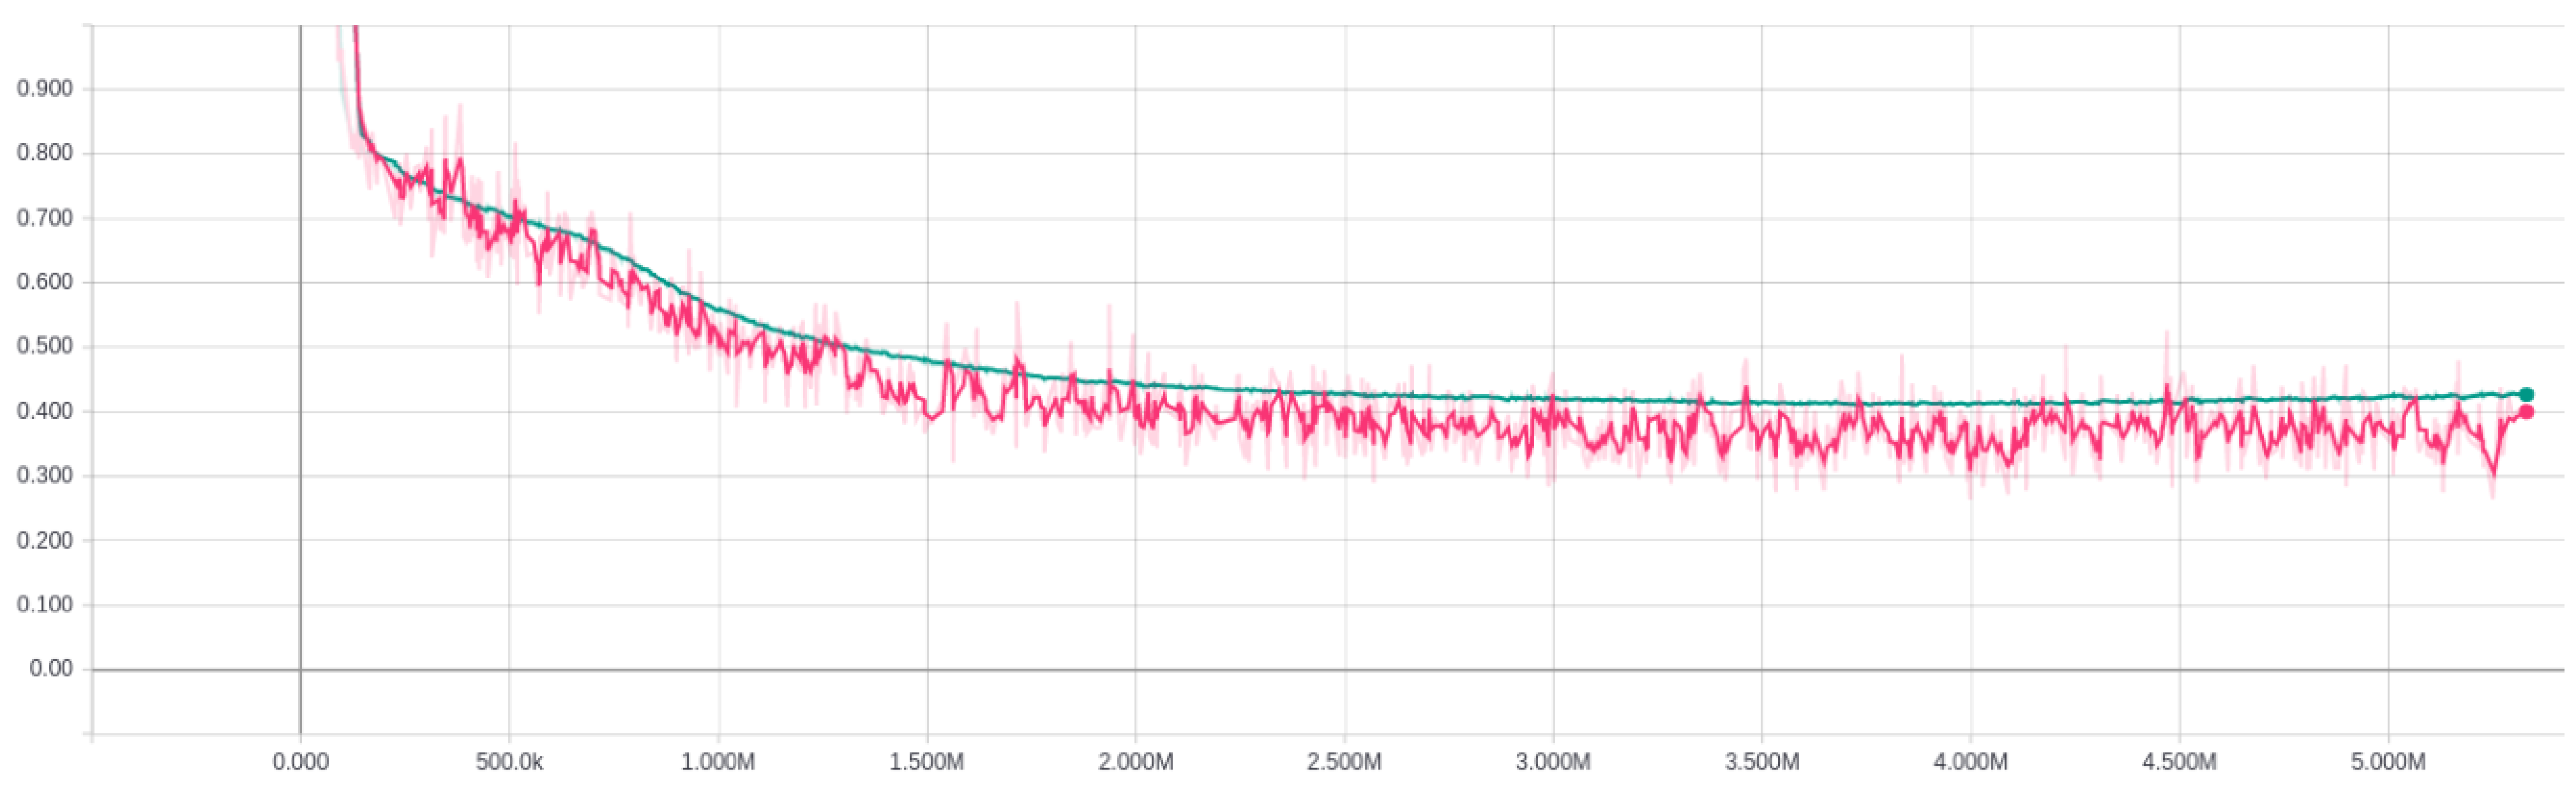
\includegraphics[width=\linewidth]{figures/nopretrained_50_50.eps}
  \caption{Cross-entropy error (Y-axis) on the training (red) and validation (green) sets of a 2-hidden-layer, 50 neurons each, fully connected network, called $A_0$, with randomly initialized weights and biases. Notice that the validation curve started to go up after about $3.8$ millions of batch updates, indicating the overfitting of the network.}
  \label{fig:nopretrained_50_50}
\end{figure}

Figure~\ref{fig:stack_50_50_dropout_elu_learning_curves} shows the learning curves for a similar stack as above but the two denoising autoencoders were pretrained to reconstruct their inputs, and the resulting weights and biases were used to initialize the stack before being fine-tuned. We could observe that the network did not overfit even after more than $18$ millions batch updates, which is much better than $A_0$. The cross-entropy error of this network on the validation set can also be seen as much better than from the one with randomly initialized weights and biases: less than $0.3$ vs. greater than $0.4$. This by definition results in a difference between $A_1$ and $A_0$ in terms of prediction accuracy on the validation, and importantly, the \emph{test} sets: $90.34\%$ vs. $87.52\%$, respectively. The accuracy errors by the two networks on the various sets are shown in Table~\ref{tab:Accuracy_A0_vs_A1}.

\begin{table}
\begin{center}
\begin{tabular}{|l||c|c|c|}
\hline
Network & Train set & Validation set & Test set \\ \hline \hline
$A_0$ & $89.59\%$ & $87\%$ & $87.52\%$ \\ \hline
$A_1$ & $93.17\%$ & $88.96\%$ & $90.34\%$ \\ \hline
\end{tabular}
\caption{Accuracy by networks $A_0$ and $A_1$ on training, validation and test sets.}
\label{tab:Accuracy_A0_vs_A1}
\end{center}
\end{table}

Although the network $A_1$ had a wider accuracy gap between its training and validation sets, it is important to stress that this gap did not appear to be widening, which was not the case for the network $A_0$. If the training were to be allowed on $A_1$, we would expect that its generalization capacity continues to be enhanced; the network $A_0$, however, overfitted early and would not have any benefits from further training.

\begin{figure}
  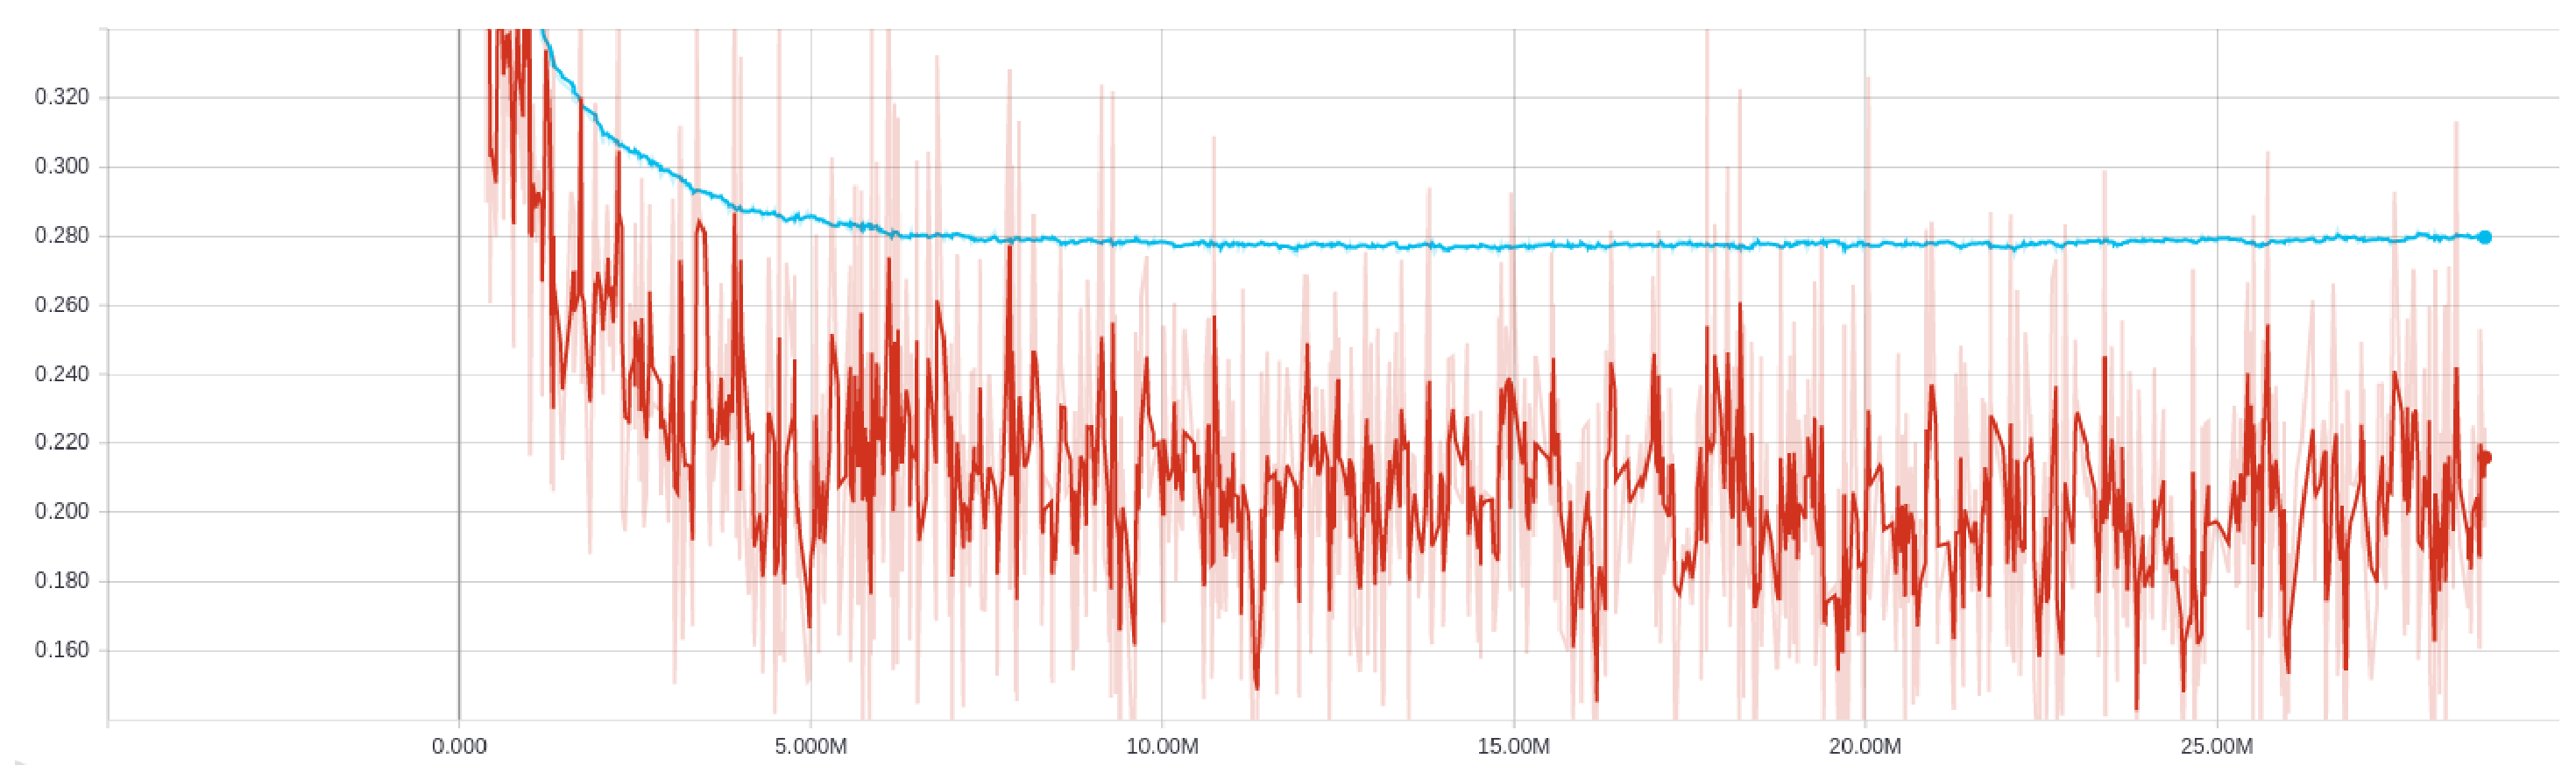
\includegraphics[width=\linewidth]{figures/stack_50_50_dropout_elu/learning_curves.eps}
  \caption{Cross-entropy error (Y-axis) on the training (red) and validation (green) sets of a 2-hidden-layer fully connected network, called $A_1$, whose weights and biases were initialized with pretrained values.}
  \label{fig:stack_50_50_dropout_elu_learning_curves}
\end{figure}

\vspace{5mm}
\noindent
\textbf{B. Traditional vs. denoising autoencoders:}
\noindent
We now compare two types of autoencoders, traditional and denoising, in terms of reconstructing orginal inputs and, more importantly, of learning representations for our classification problem. The denoising autoencoders here were those used to pretrain weights/biases of $A_1$, which learned their unique features by reconstructing the inputs from their corrupted version. The traditional autoencoders had the same configuration with the other type (i.e., number of neurons, dropout rates for the hidden layer), except that they attempted to reconstruct the inputs from themself instead of their corrupted version. To test their representations in classifying the target signals, we constructed a 2-hidden-layer fully-connected neural network, called $B_0$, whose weights and biases were initialized from the two pretrained traditional autoencoders. No Gaussian noises or dropout was applied to the inputs of the network $B_0$.

Table~\ref{tab:reconstruction_errors} shows the reconstruction errors by two autoencoders of the above types used to construct the layers of networks $A_1$ and $B_0$. On both the training and validation sets, the traditional autoencoders which processed the inputs directly resulted in more accurate reconstructed signals, i.e. with smaller errors, than those produced by the denoising counterpart; and this is true for autoencoders corresponding to both two hidden layers of the networks.

\begin{table}[!htbp]
\centering
\begin{tabular}{*5c}
\toprule
Autoencoder &  \multicolumn{2}{c}{Layer 1} & \multicolumn{2}{c}{Layer 2}\\
\midrule
{}         & Train   & Validation    & Train   & Validation\\
Traditional   & 0.0015  & 0.0016   & 0.00051  & 0.00052\\
Denoise    &  0.0019  &  0.0021   & 0.0011  & 0.0011\\
\bottomrule
\end{tabular}
\caption{Reconstruction errors by traditional and denoise autoencoders used at layer 1 and 2 of networks $B_0$ and $A_1$, respectively.}
\label{tab:reconstruction_errors}
\end{table}

Figure~\ref{fig:reconstructed_inputs_comparison} shows the 522th segment and its reconstructed signals produced by networks $B_0$ and $A_1$. We can notice that at around the dimension 150th, the signal generated by the network $B_0$ shows more accurate reconstructed curve than that of $A_1$. This observation can be seen with other segments and their reconstructed signals, consistent with the comparison above between the networks in terms of their reconstructed errors.
\begin{figure}
\begin{subfigure}{.5\textwidth}
  \centering
  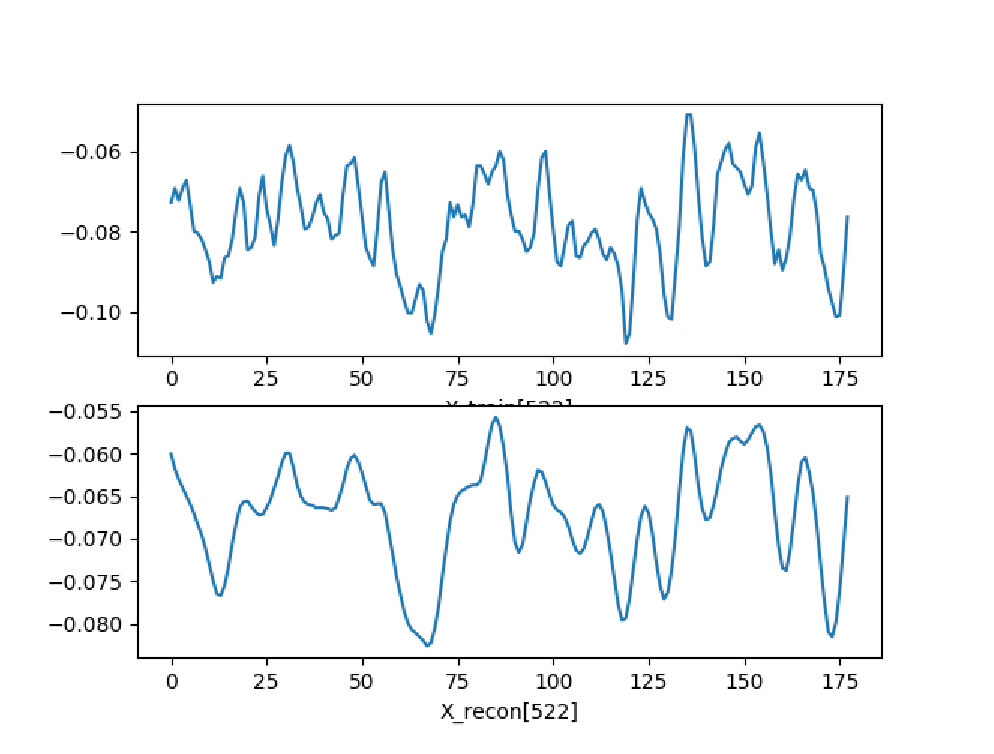
\includegraphics[width=.8\linewidth]{figures/clean_input_example_522.eps}
\end{subfigure}%
~
\begin{subfigure}{.5\textwidth}
  \centering
  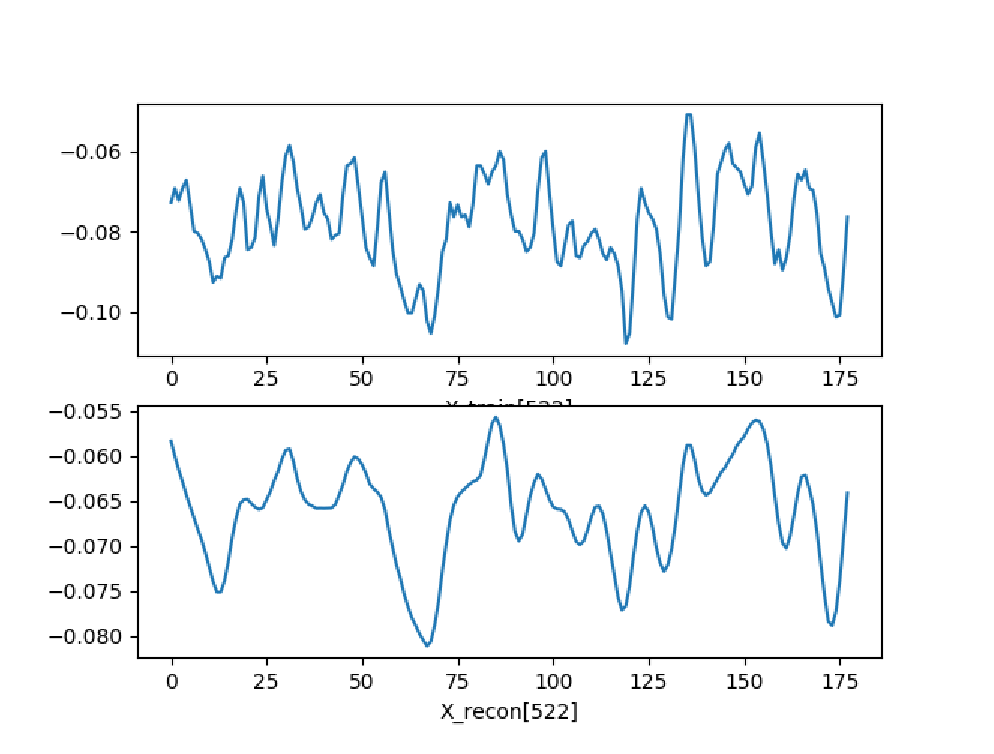
\includegraphics[width=.8\linewidth]{figures/corrupted_input_example_522.eps}
\end{subfigure}
\caption{Segment 522th and its reconstructed signals produced by networks $B_0$ (left) and $A_1$ (right).}
\label{fig:reconstructed_inputs_comparison}
\end{figure}

The outperformance of traditional autoencoders in reconstructing the input signals, however, did not transform to its classification performance. Figure~\ref{fig:stack_50_50_dropout_elu_clean_input} shows the cross-entropy errors by the network $B_0$: it was expressive enough and achieved $97.13\%$ accuracy on the training set, however overfitted early after step $1,675,620$ of batch updates. The accuracy of the resulting best model on the validation and testing sets were $90.47\%$ and $91.78\%$, respectively. (The corresponding statistics by $A_1$ was presented in the previous result section.) Both the about $7\%$ performance gaps on between the training and the two independent sets, and the $>1\%$ gap between the validation and test sets indicate that this model suffers from high variance. The network $A_1$, which used features extracted through reconstructing corrupted inputs, as shown in Figure~\ref{fig:stack_50_50_dropout_elu_learning_curves}, provided a comparable and more reliable accuracy performance on unseen data.

\begin{figure}
  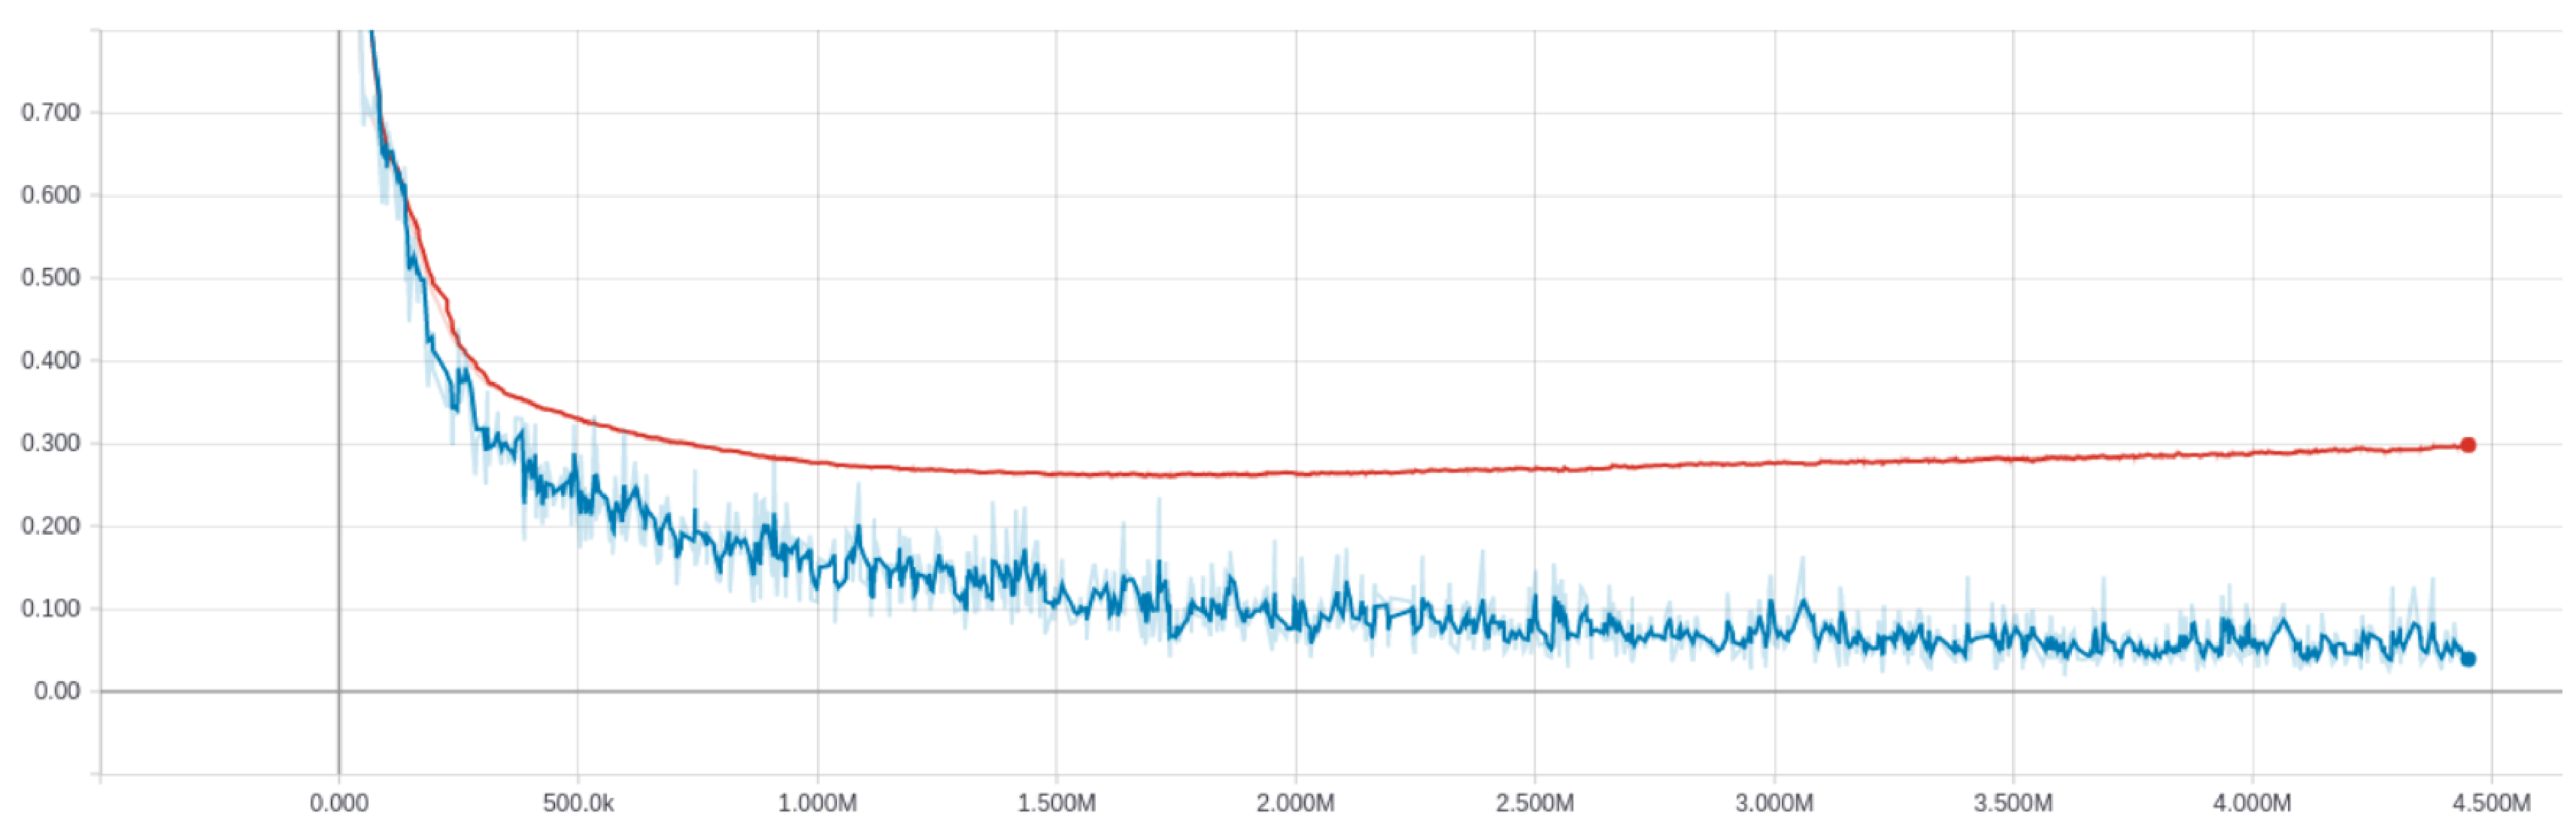
\includegraphics[width=\linewidth]{figures/stack_50_50_dropout_elu_clean_input/stack_50_50_dropout_elu_clean_input.eps}
  \caption{Cross-entropy error (Y-axis) on the training (green) and validation (red) sets of a 2-layer fully connected network, called $B_0$, with inputs not being corrupted during training.}
  \label{fig:stack_50_50_dropout_elu_clean_input}
\end{figure}

Perhaps one explanation for the above difference could be that since the two networks were the same except for the clean vs. the corrupted inputs that they processed, the noises introduced into the inputs helped the network $A_1$ learned features more essential to the original inputs; when used for classification task, these features resulted in much less overfitting model compared to those simply learned from an identity function of the clean inputs. Although it is hard for humans to make sense the features learned by the two networks to represent brain activity signals (in contrast to interpretable features in image domains), it is interesting to see what the neurons were ``excited'' about after the learning process. Figure~\ref{fig:weights_stack_50_50_dropout_elu_clean_input} shows the weights of six randomly chosen neurons learned by the first traditional autoencoder used in network $B_0$: we could observe that the weights did not appear to learn any interesting patterns after reconstructing the original inputs.

\begin{figure}
\begin{subfigure}{.5\textwidth}
  \centering
  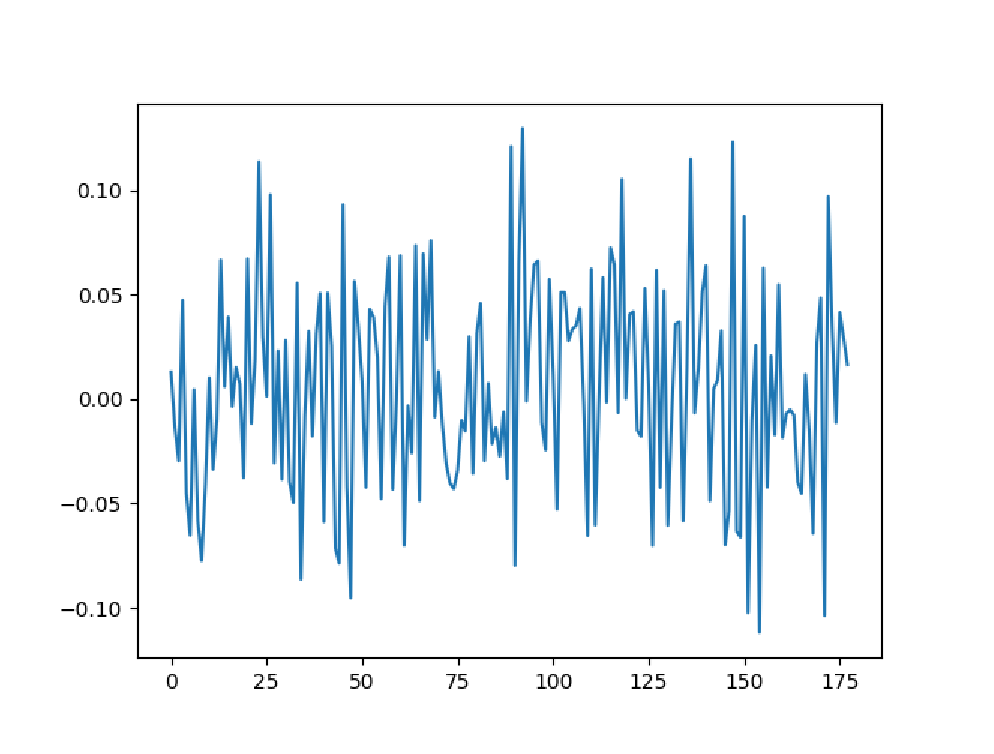
\includegraphics[width=.8\linewidth]{figures/stack_50_50_dropout_elu_clean_input/weights_neuron_0.eps}
\end{subfigure}%
\begin{subfigure}{.5\textwidth}
  \centering
  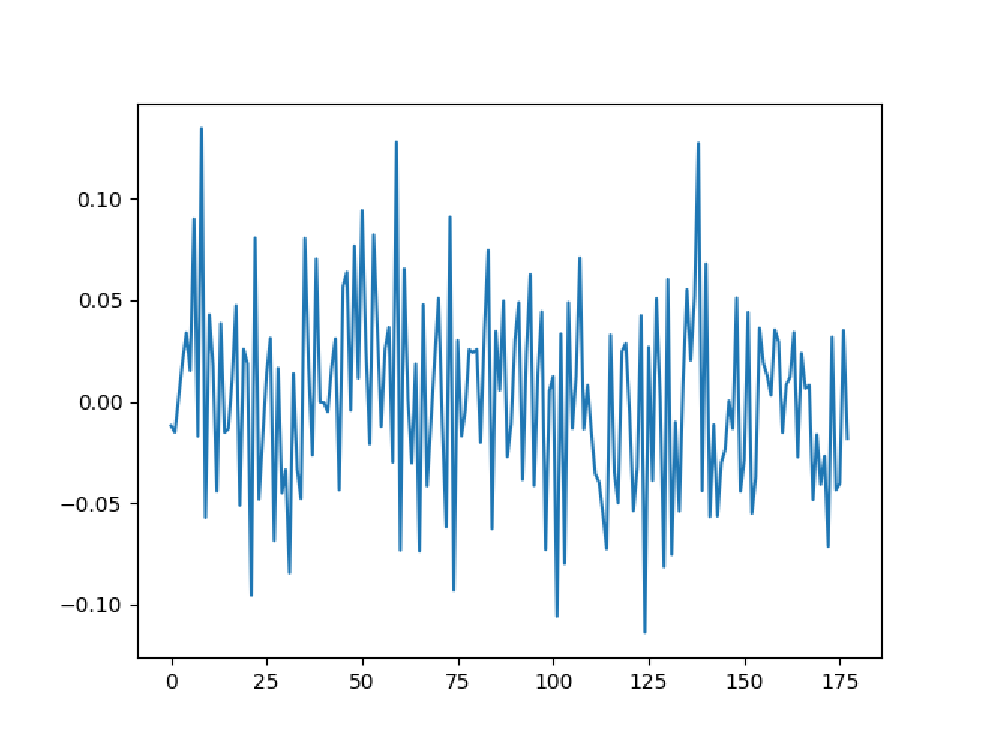
\includegraphics[width=.8\linewidth]{figures/stack_50_50_dropout_elu_clean_input/weights_neuron_1.eps}
\end{subfigure}

\begin{subfigure}{.5\textwidth}
  \centering
  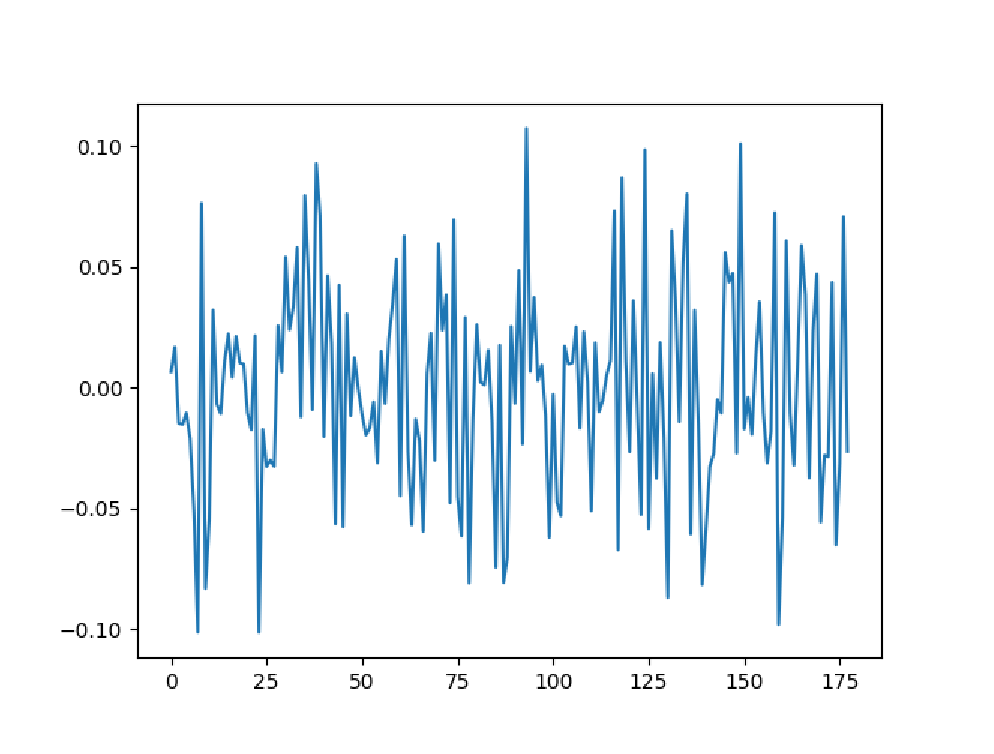
\includegraphics[width=.8\linewidth]{figures/stack_50_50_dropout_elu_clean_input/weights_neuron_2.eps}
\end{subfigure}%
\begin{subfigure}{.5\textwidth}
  \centering
  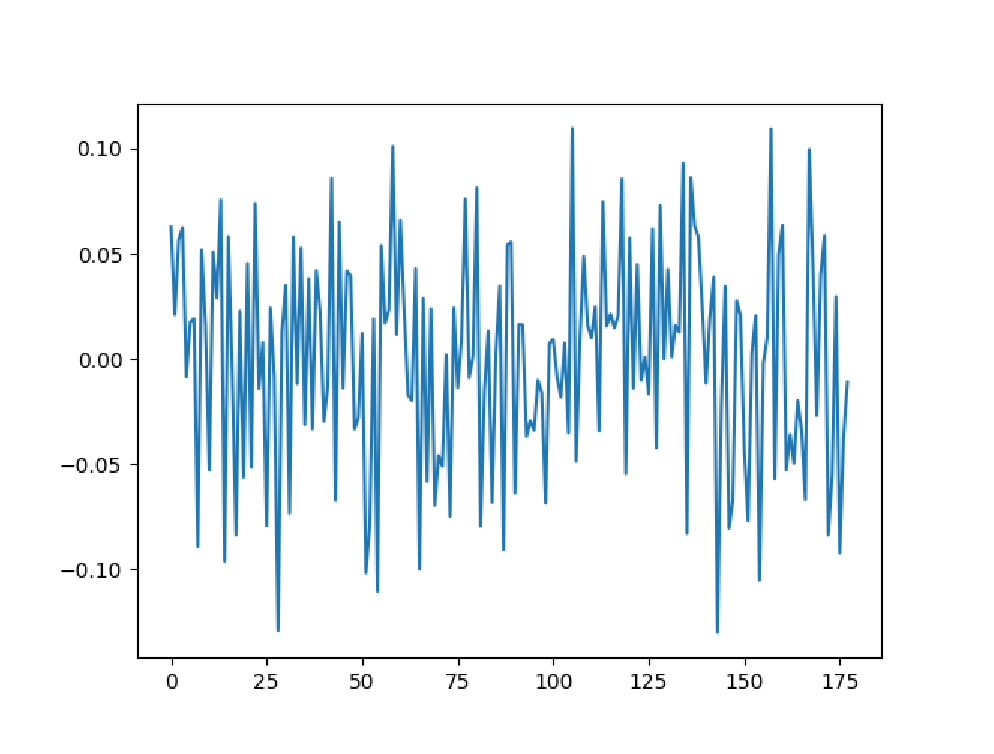
\includegraphics[width=.8\linewidth]{figures/stack_50_50_dropout_elu_clean_input/weights_neuron_3.eps}
\end{subfigure}

\begin{subfigure}{.5\textwidth}
  \centering
  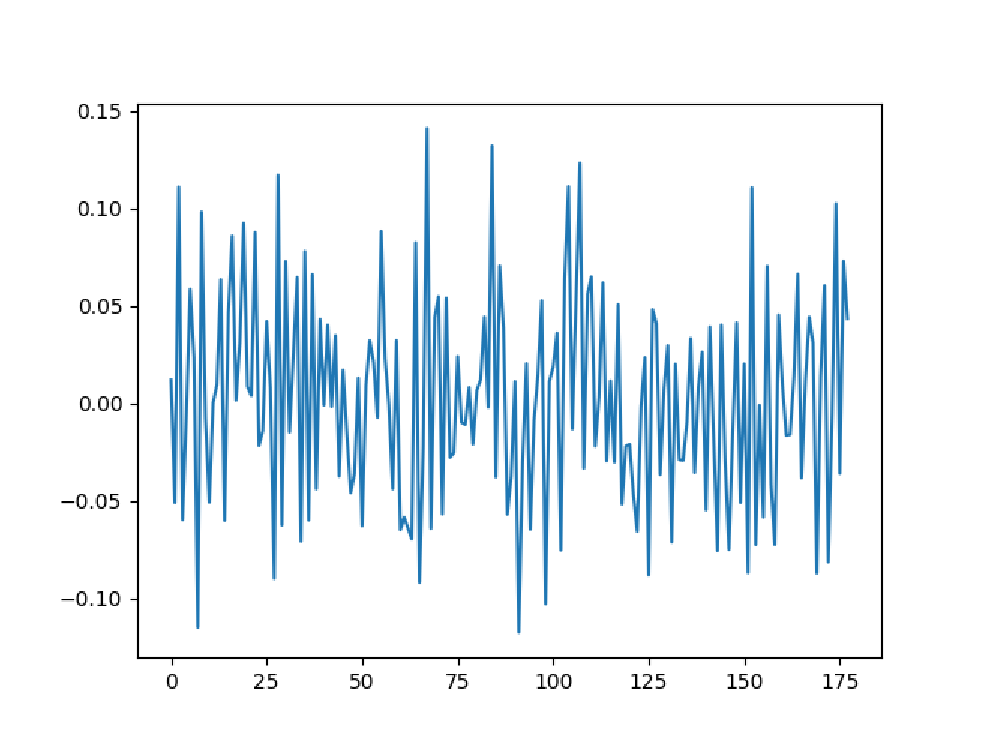
\includegraphics[width=.8\linewidth]{figures/stack_50_50_dropout_elu_clean_input/weights_neuron_4.eps}
\end{subfigure}
\begin{subfigure}{.5\textwidth}
  \centering
  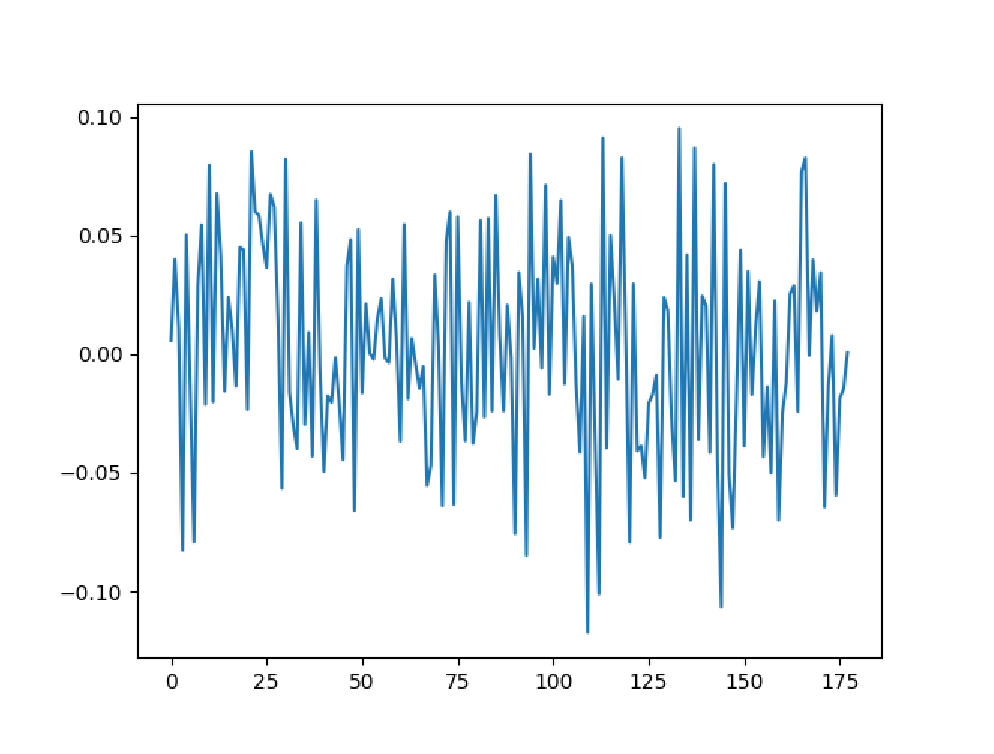
\includegraphics[width=.8\linewidth]{figures/stack_50_50_dropout_elu_clean_input/weights_neuron_8.eps}
\end{subfigure}
\caption{Weights of six neurons, chosen randomly, learned by the first traditional autoencoder used in network $B_0$ after reconstructing the original (uncorrupted) inputs.}
\label{fig:weights_stack_50_50_dropout_elu_clean_input}
\end{figure}

For the same set of neurons, Figure~\ref{fig:weights_stack_50_50_dropout_elu} shows their weights learned by the denoising autoencoder used in the first hidden layer of network $A_1$ after reconstructing the inputs from their corrupted version. As opposed to those in Figure~\ref{fig:weights_stack_50_50_dropout_elu_clean_input}, these weights appear to reflect some specific patterns that the neurons were adapted to. Similar contrasts could also be observed for autoencoders at the second layers of the networks $B_0$ and $A_1$.

\begin{figure}
\begin{subfigure}{.5\textwidth}
  \centering
  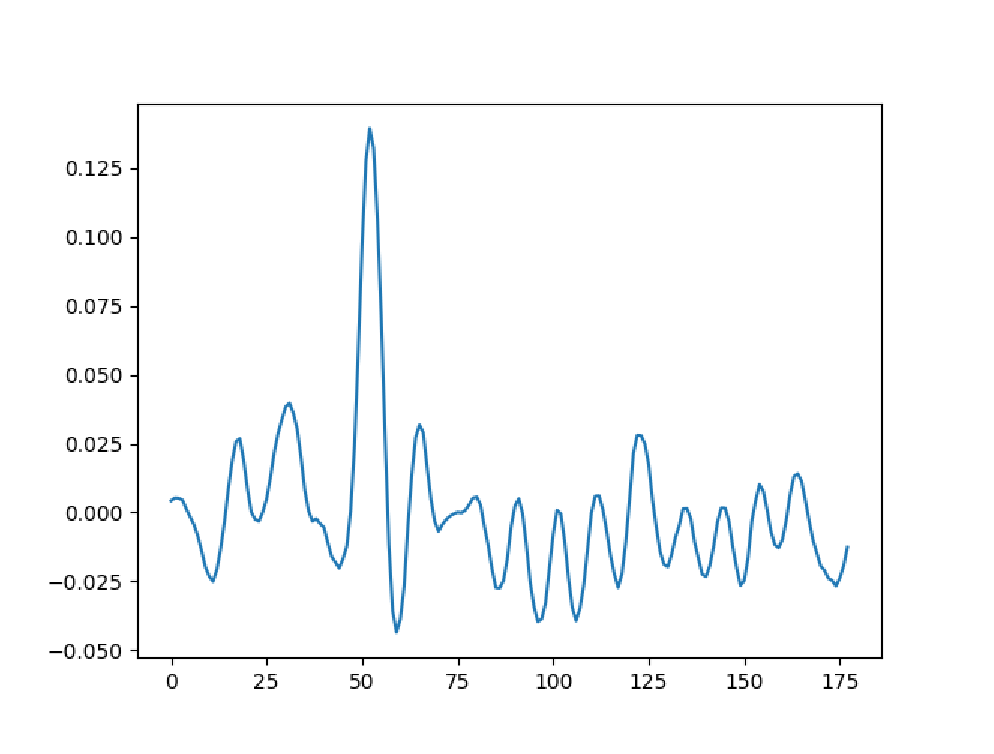
\includegraphics[width=.8\linewidth]{figures/stack_50_50_dropout_elu/weights_neuron_0.eps}
\end{subfigure}%
\begin{subfigure}{.5\textwidth}
  \centering
  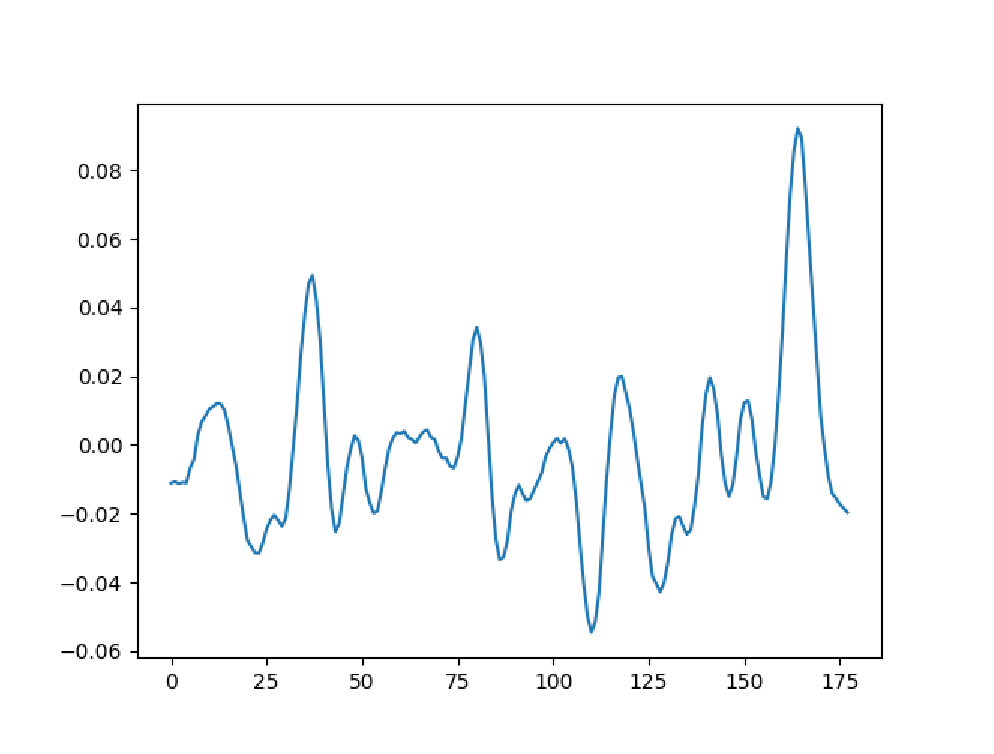
\includegraphics[width=.8\linewidth]{figures/stack_50_50_dropout_elu/weights_neuron_1.eps}
\end{subfigure}

\begin{subfigure}{.5\textwidth}
  \centering
  \includegraphics[width=.8\linewidth]{figures/stack_50_50_dropout_elu/weights_neuron_2.eps}
\end{subfigure}%
\begin{subfigure}{.5\textwidth}
  \centering
  \includegraphics[width=.8\linewidth]{figures/stack_50_50_dropout_elu/weights_neuron_3.eps}
\end{subfigure}

\begin{subfigure}{.5\textwidth}
  \centering
  \includegraphics[width=.8\linewidth]{figures/stack_50_50_dropout_elu/weights_neuron_4.eps}
\end{subfigure}
\begin{subfigure}{.5\textwidth}
  \centering
  \includegraphics[width=.8\linewidth]{figures/stack_50_50_dropout_elu/weights_neuron_8.eps}
\end{subfigure}
\caption{Weights of the corresponding six neurons in Figure~\ref{fig:weights_stack_50_50_dropout_elu_clean_input} learned by the first denoising autoencoder used in network $A_1$ after reconstructing the corrupted inputs.}
\label{fig:weights_stack_50_50_dropout_elu}
\end{figure}

\textit{Comparison on networks of 75-neuron layers}: Table~\ref{tab:Accuracy_B1_vs_B2} shows the accuracy performances of networks $B_1$ and $B_2$ with 2-hidden-layer fully connected networks, each having 75 neurons. They differed in exactly the same way $B_0$ and $A_1$ were distinguished: $B_1$ reconstructed the original signals from clean inputs, whereas $B_2$ did that from the corrupted inputs. We can again observe from the accuracy gaps that by reconstructing the inputs from their corrupted version, the denoising autoencoders extracted features that helped the network classifier learned a model that was more reliable in predicting the target classes.

\begin{table}
\begin{center}
\begin{tabular}{|l||c|c|c|l|}
\hline
Network & Train set & Validation set & Test set\\ \hline \hline
$B_1$ & $97.3\%$ & $89.61\%$ & $90.22\%$\\ \hline
$B_2$ & $94.28\%$ & $89.99\%$ & $90.69\%$\\ \hline
\end{tabular}
\caption{Accuracy by networks with 2 layers of 75 neurons $B_1$ and $B_2$ on training, validation and test sets. $B_1$ reconstructed the original signals from themselves, and $B_2$ did so from the corrupted inputs.}
\label{tab:Accuracy_B1_vs_B2}
\end{center}
\end{table}

\vspace{5mm}
\noindent
\textbf{C. Gaussian noisy inputs vs. dropout inputs:}

\noindent
I found that using Gaussian noises to corrupt the inputs of autoencoders seemed to work equally well compared to using the dropout technique. Figure~\ref{fig:stack_50_50_noise0.1_elu} shows the learning curves on the training and validation sets produced by a network, called $C_0$, that is similar to $A_1$ except for inputs being corrupted using Gaussian noises of 0.1 standard deviation (instead of dropout with rate $0.33$ used by $A_1$ and its autoencoders.) The best model by $C_0$ was saved at step $17,575,820$ of batch updates, after which the performance on the validation set started to decrease indicating that the model began to overfit to the training data. The accuracy performance of $C_0$, compared to $A_1$, is summarized in Table~\ref{tab:Accuracy_C0_vs_A1}.

\begin{figure}
  \includegraphics[width=\linewidth]{figures/stack_50_50_noise0.1_elu/learning_curves.eps}
  \caption{Cross-entropy error (Y-axis) on the training (red) and validation (green) sets of a network, called $C_0$, that is similar to $A_1$ except for the inputs being corrupted using Gaussian noises instead of dropout.}
  \label{fig:stack_50_50_noise0.1_elu}
\end{figure}

\begin{table}
\begin{center}
\begin{tabular}{|l||c|c|c|l|}
\hline
Network & Train set & Validation set & Test set\\ \hline \hline
$C_0$ & $93.84\%$ & $90.43\%$ & $90.52\%$\\ \hline
$A_1$ & $93.17\%$ & $88.96\%$ & $90.34\%$ \\ \hline
\end{tabular}
\caption{Accuracy by networks $C_0$ and $A_1$ representing the effects of using Gaussian noises and dropout to corrupt the inputs for learning representations.}
\label{tab:Accuracy_C0_vs_A1}
\end{center}
\end{table}

\vspace{5mm}
\noindent
\textbf{D. Denoising autoencoders with dropout: number of neurons and layers}

\noindent
\textit{Number of hidden neurons:} Table~\ref{tab:Accuracy_diff_num_neurons} shows the accuracy performance on the three sets of 2-hidden-layer networks with different number of hidden neurons. We can see that increasing the size of the hidden layers from $50$ to $75$ and to $100$ improved the accuracy up to $1\%$; unfortunately the performance gaps between training and validation/test sets also got wider, increasing the variances of the bigger networks. With $250$ hidden neurons (network $D_1$), the network achieved $99.42\%$ accuracy on the training set but did not improve much on the independent test set ($91.95\%$). As shown in Figure~\ref{fig:stack_250_250_dropout_elu}, this network overfitted to the training set at step $6,073,855$ of batch updates. For that many hidden neurons, perhaps a more agressive dropout would be needed to cope with overfitting.

\begin{table}
\begin{center}
\begin{tabular}{|l||c|c|c|l|}
\hline
Network & \#Neurons/layer & Train set & Validation set & Test set\\ \hline \hline
$A_1$ & $50$ & $93.17\%$ & $88.96\%$ & $90.34\%$ \\ \hline
$B_2$ & $75$ & $94.27\%$ & $89.99\%$ & $90.69\%$ \\ \hline
$D_0$ & $100$ & $95.68\%$ & $90.56\%$ & $91.52\%$ \\ \hline
$D_1$ & $250$ & $99.42\%$ & $90.95\%$ & $91.95\%$ \\ \hline
\end{tabular}
\caption{Accuracy by networks of two hidden layers with different number of neurons per layer.}
\label{tab:Accuracy_diff_num_neurons}
\end{center}
\end{table}

\begin{figure}
  \includegraphics[width=\linewidth]{figures/stack_250_250_dropout_elu/learning_curves.eps}
  \caption{Cross-entropy error (Y-axis) on the training (red) and validation (green) sets of 2-hidden-layer network $D_1$ which has $250$ hidden neurons per layer.}
  \label{fig:stack_250_250_dropout_elu}
\end{figure}

\vspace{5mm}
\noindent
\textit{Number of hidden layers:} As shown above for 2-hidden-layer networks, increasing number of hidden neurons could help with improving the accuracy performance (though not much unless more agressive ways were used to deal with overfitting). The number of hidden layers is also another hyperparamter that determines the expressiveness of a neural network. With our small training set of about $6900$ examples, we might not need much deeper neural network. Figure~\ref{fig:stack_50} and \ref{fig:stack_50_50_50} shows the learning curves by networks of 1 and 3 hidden layers, each of which has 50 hidden neurons, and Table~\ref{tab:stack_50_50_50} shows the accuracy performance on the training, validation and testing sets of these networks compared to their counterpart that has 2 hidden layers. We can observe that their performance are quite close with $A_1$, which has 2 hidden layers, being slightly better than the others on an independent test set.

\begin{figure}
  \includegraphics[width=\linewidth]{figures/stack_50_dropout_elu/learning_curves.eps}
  \caption{Cross-entropy error (Y-axis) on the training (red) and validation (green) sets of a network, called $D_2$, that is similar to $A_1$ but has 1 hidden layer.}
  \label{fig:stack_50}
\end{figure}

\begin{figure}
  \includegraphics[width=\linewidth]{figures/stack_50_50_50_dropout_elu/learning_curves.eps}
  \caption{Cross-entropy error (Y-axis) on the training (red) and validation (green) sets of a network, called $D_3$, that is similar to $A_1$ but has 3 hidden layers.}
  \label{fig:stack_50_50_50}
\end{figure}

\begin{table}
\begin{center}
\begin{tabular}{|l||c|c|c|l|}
\hline
Network & \#Hidden layers & Train set & Validation set & Test set\\ \hline \hline
$D_2$ & $1$ & $93.34\%$ & $89.26\%$ & $89.43\%$\\ \hline
$A_1$ & $2$ & $93.17\%$ & $88.96\%$ & $90.34\%$ \\ \hline
$D_3$ & $3$ & $92.98\%$ & $88.56\%$ & $89.69\%$\\ \hline
\end{tabular}
\caption{Accuracy by networks of 1, 2 and 3 hidden layers with 50 hidden neurons per layer.}
\label{tab:stack_50_50_50}
\end{center}
\end{table}

\vspace{5mm}
\noindent
\textit{External comparison}: As mentioned earlier, the work by Kabir et al.~\cite{kabir2016epileptic} achieved an accuracy of $95.3\%$ on an independent test set. The best performance I could get from training various network configurations is about $90.34\%$ to $91.52\%$ (with 2-hidden layer networks of $50$ and $75$ neurons per hidden layer), which in my opinion is very encouraging for an approach that learns features automatically. One important difference between my work and the one by Kabir et al.~\cite{kabir2016epileptic} is that their approach required the original 23.6-second channels to be divided into 5.9-second segments, more than 5 times longer than those used in the present approach. Their method, which was based on computing special statistics from those 5.9-second segments, might need such long segments in order to gather enough information for classification.

\section{Conclusion}

\noindent
This work presented an approach to classifying brain activitiy signals in the data set provided by ~\cite{andrzejak2001indications} into volunteer classes related to epileptic seizure disease. The proposed method and results can be summarized as follows:
\begin{itemize}
\item Two types of autoencoders, traditional and denoising, were used to learn representations of the original signal segments.
\item The encoding parts of the autoencoders were then put together to form the hidden layers of a multi-layer feed-forward neural network.
\item The network was then fine-tuned to classify three classes of volunteers.
\item The performances of the network on an independet test set vary from $90.34\%$ to $91.52\%$, obtained from networks with 2 hidden layers with 50 to 70 neurons per layer. These network configurations appeared to converge with stable gaps between training and validation performances. Although this accuracy result is lower than the work by Kabir et al.~\cite{kabir2016epileptic} on the same target classes, this work used much smaller 1-second segments, making it more sensitive to be used in potential applications such as medical wearable devices.
\end{itemize}

I learned valuable lessons from this project:
\begin{itemize}
\item This is the first time I learned to use TensorFlow directly (instead of through Keras). I also found Tensorboard very helpful in observing the training process.
\item I learned to recognize when the network appeared to overfit to the training data set. I also learned how to first test the capacity of the network (by not putting in any dropout rates), and then how to cope with overfitting.
\end{itemize}

Due to my limited time, there are still items that I proposed but have not completed, and are worth further investigation. Future work include: 
\begin{itemize}
\item consider using other types of autoencoders such as sparse autoencoders~\cite{boureau2008sparse} and variational autoencoders~\cite{kingma2013auto} for this data set;
\item consider using other classifiers such as Decision Trees, K-Kearest Neighbors, Support Vector Machines and Boosting with the representations learned by the sequence of autoencoders;
\item compare different approaches in terms of other measures such as F1 score.
\end{itemize}


\bibliographystyle{abbrv}
\bibliography{report}

\end{document}
